\subsubsection{Sequential switching between Tent and Logistic maps (SWITCH)} \label{sssec:switch}

SWITCH may be expressed as a composition between $M_1 \circ M_2$ given by the following recurrence:
%
\[ \left\{ \begin{array}{ccc}\label{eq:seq}
x_{n+2}~=~ 4~x_{n+1}~(1-{n+1}) \\
x_{n+1}~=~ \left\{ \begin{array}{ll}
2~{x_n} & \textrm{if $0\leq x_n\leq 1/2$}\\
2~(1-{x_n}) & \textrm{if $1/2<x_n\leq 1$} 
\end{array} \right.  \end{array}\right. \] 
with $x_n\in\mathcal{R}$.
%
Results with sequential switching are shown in Figs. \ref{fig:seqdec} (a) to (f) for decimal numbers. The floating point entropy value is $H_{hist}=0.8658$, a value very similar to the one obtained for the TENT map and higher to that obtained for LOG. For decimal numbers this value is reached for $12 \leq P \leq 27$. It means it is enough to use $12$ decimal figures to get the same distribution of values in the time series. Regarding ordering patterns the number of MP decreases to $586$, a value lower lower than the one obtained for any of two simple maps TENT and LOG. It means the entropy $H_{BP}$ may increase up to $ln(134)/ln(720)\simeq 0.74$ With decimal numbers the entropy $H_{BP} $stabilizes at $P=9$ with $<H_{BP}>\simeq 0.657$ and variance $\sigma_{H_{BP}} \simeq 0.13 \times 10^{-7}$. Note that the entropies $H_{hist}$ and $H_{BP}$ are not monotonously increasing with $P$.  Considering all the quantifiers $P=12$ is the minimum number of decimal figures and statistical characteristics of this combined map are better than those for each individual map.
%
Results with sequential switching in binary numbers are shown in Figs. \ref{fig:seqbin}. Results for a number of bits $B\simeq27$ are equivalent to those obtained for $P\simeq 9$ for decimal numbers. It means both representation are valid and equivalent in the sense they will require similar hardware resources. 


\begin{figure}
	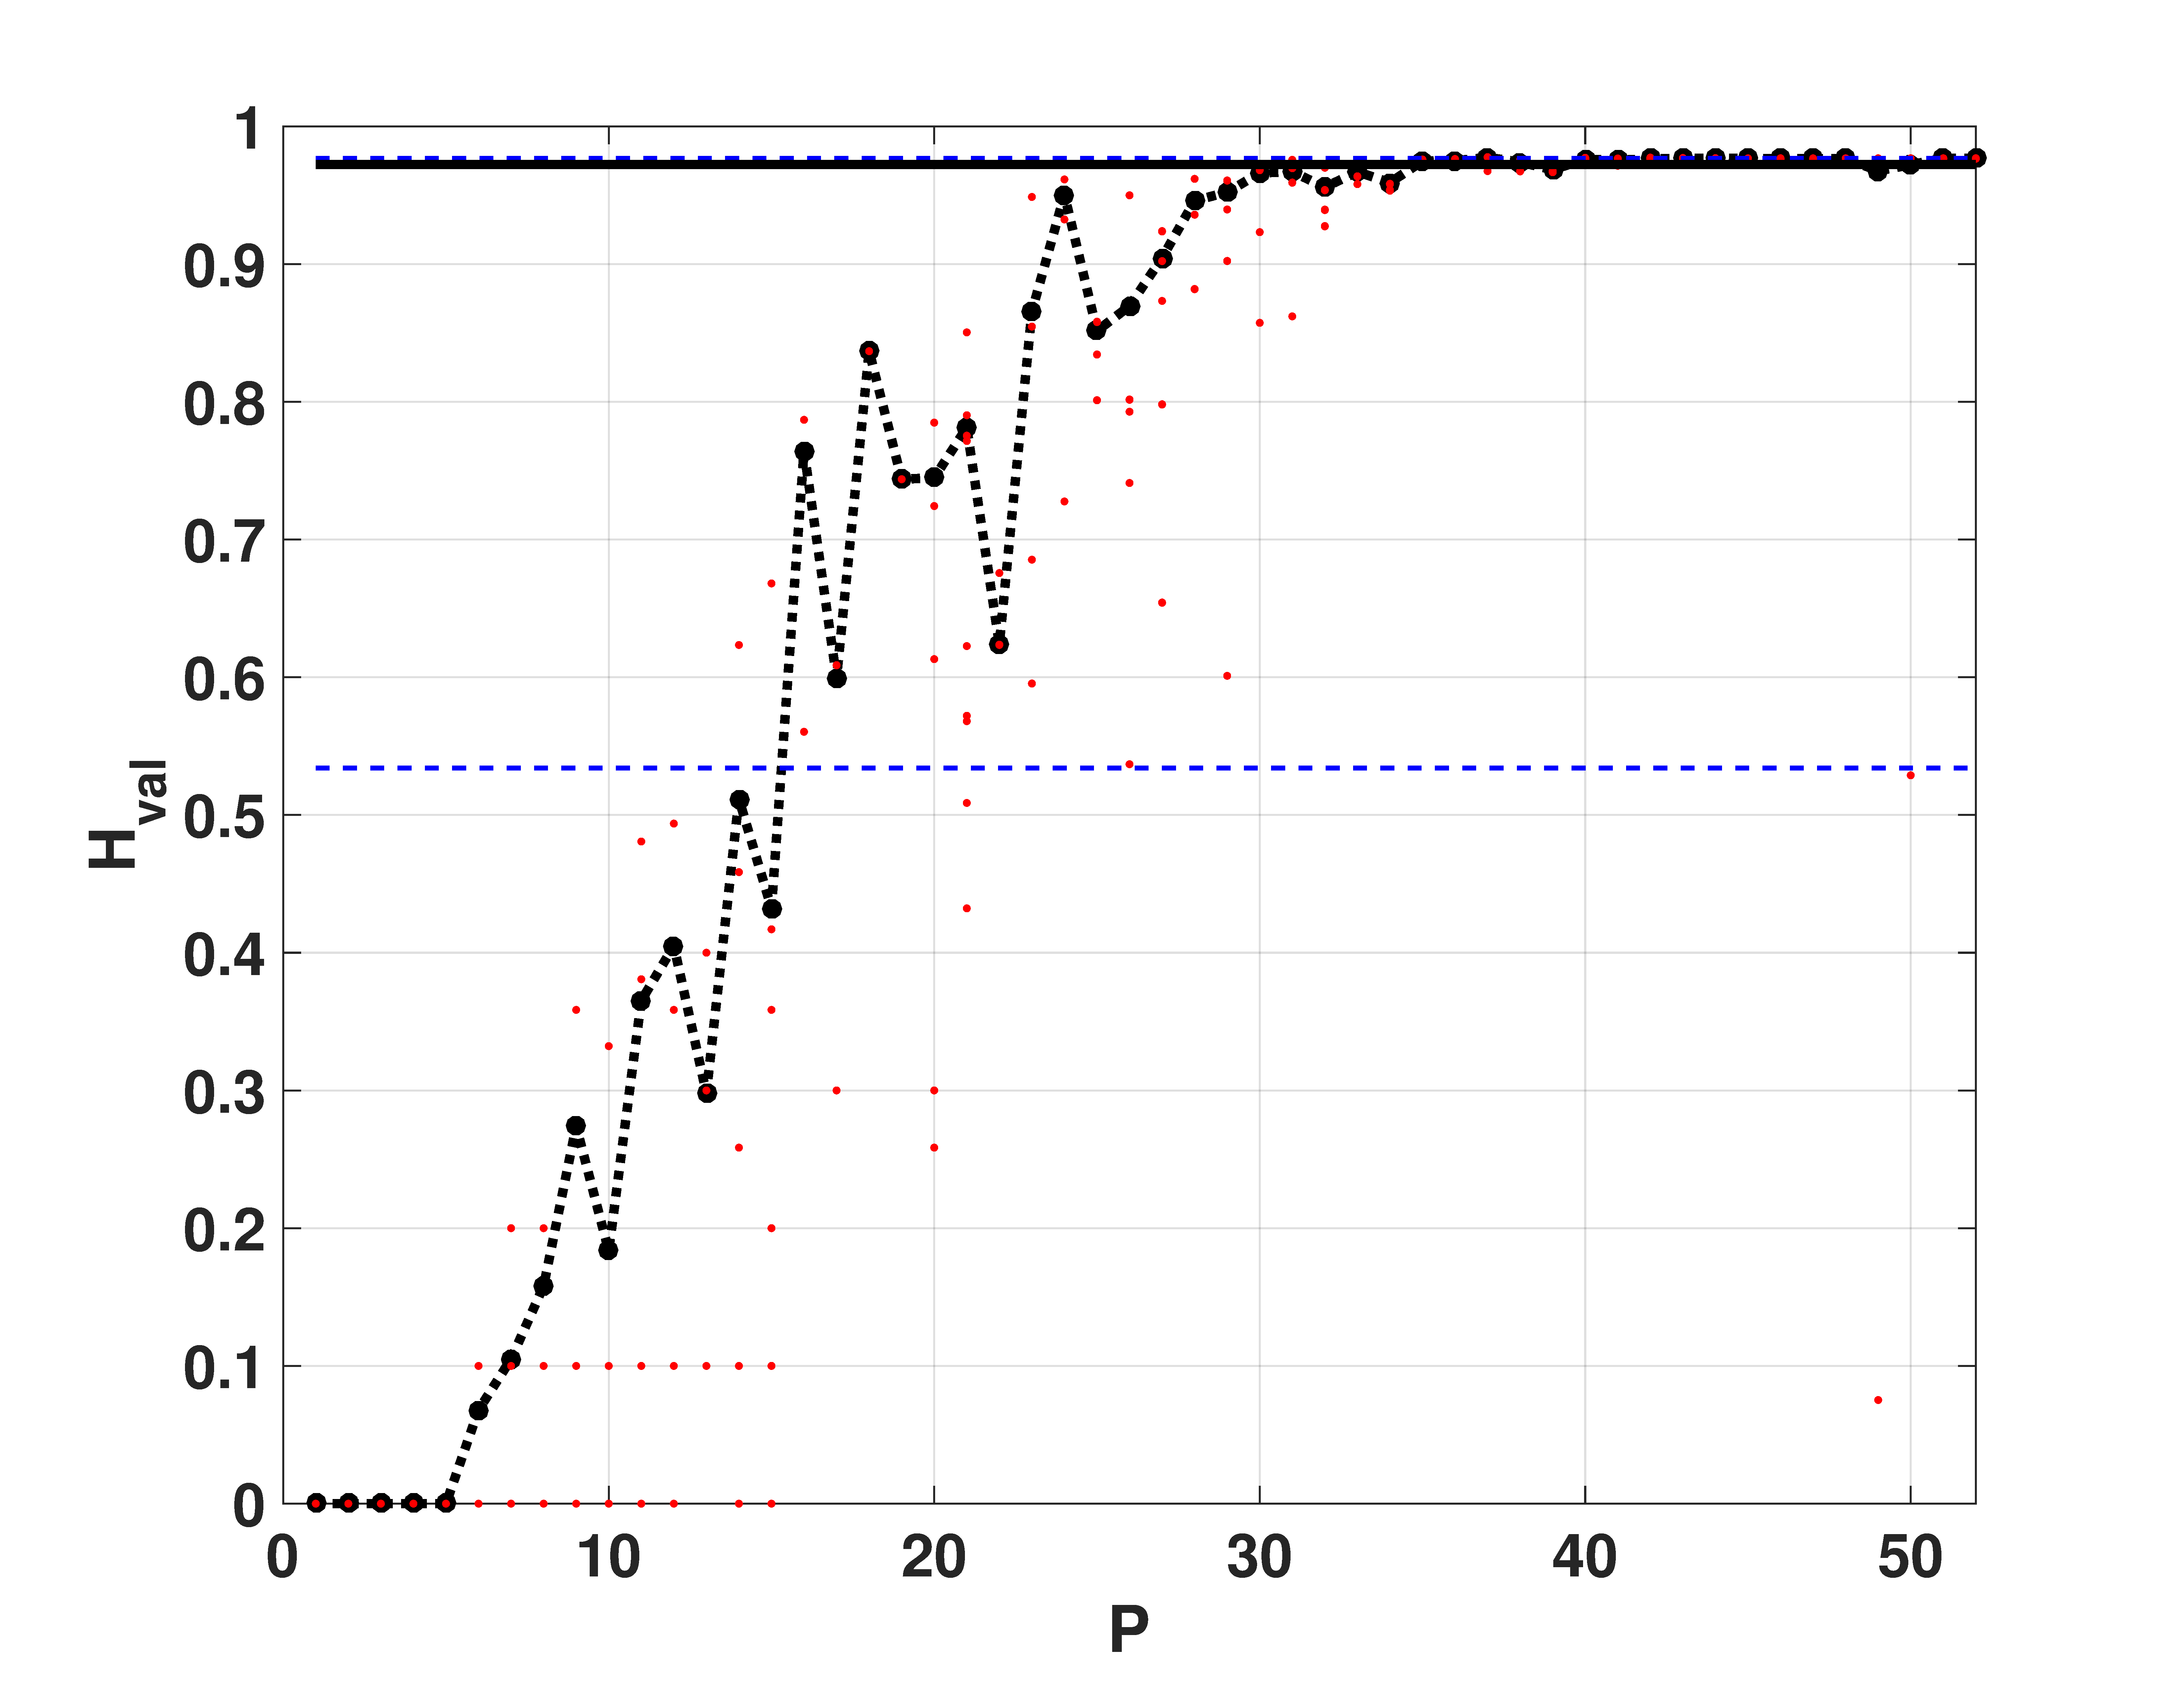
\includegraphics[width=.32\textwidth]{Hval_Switch}
	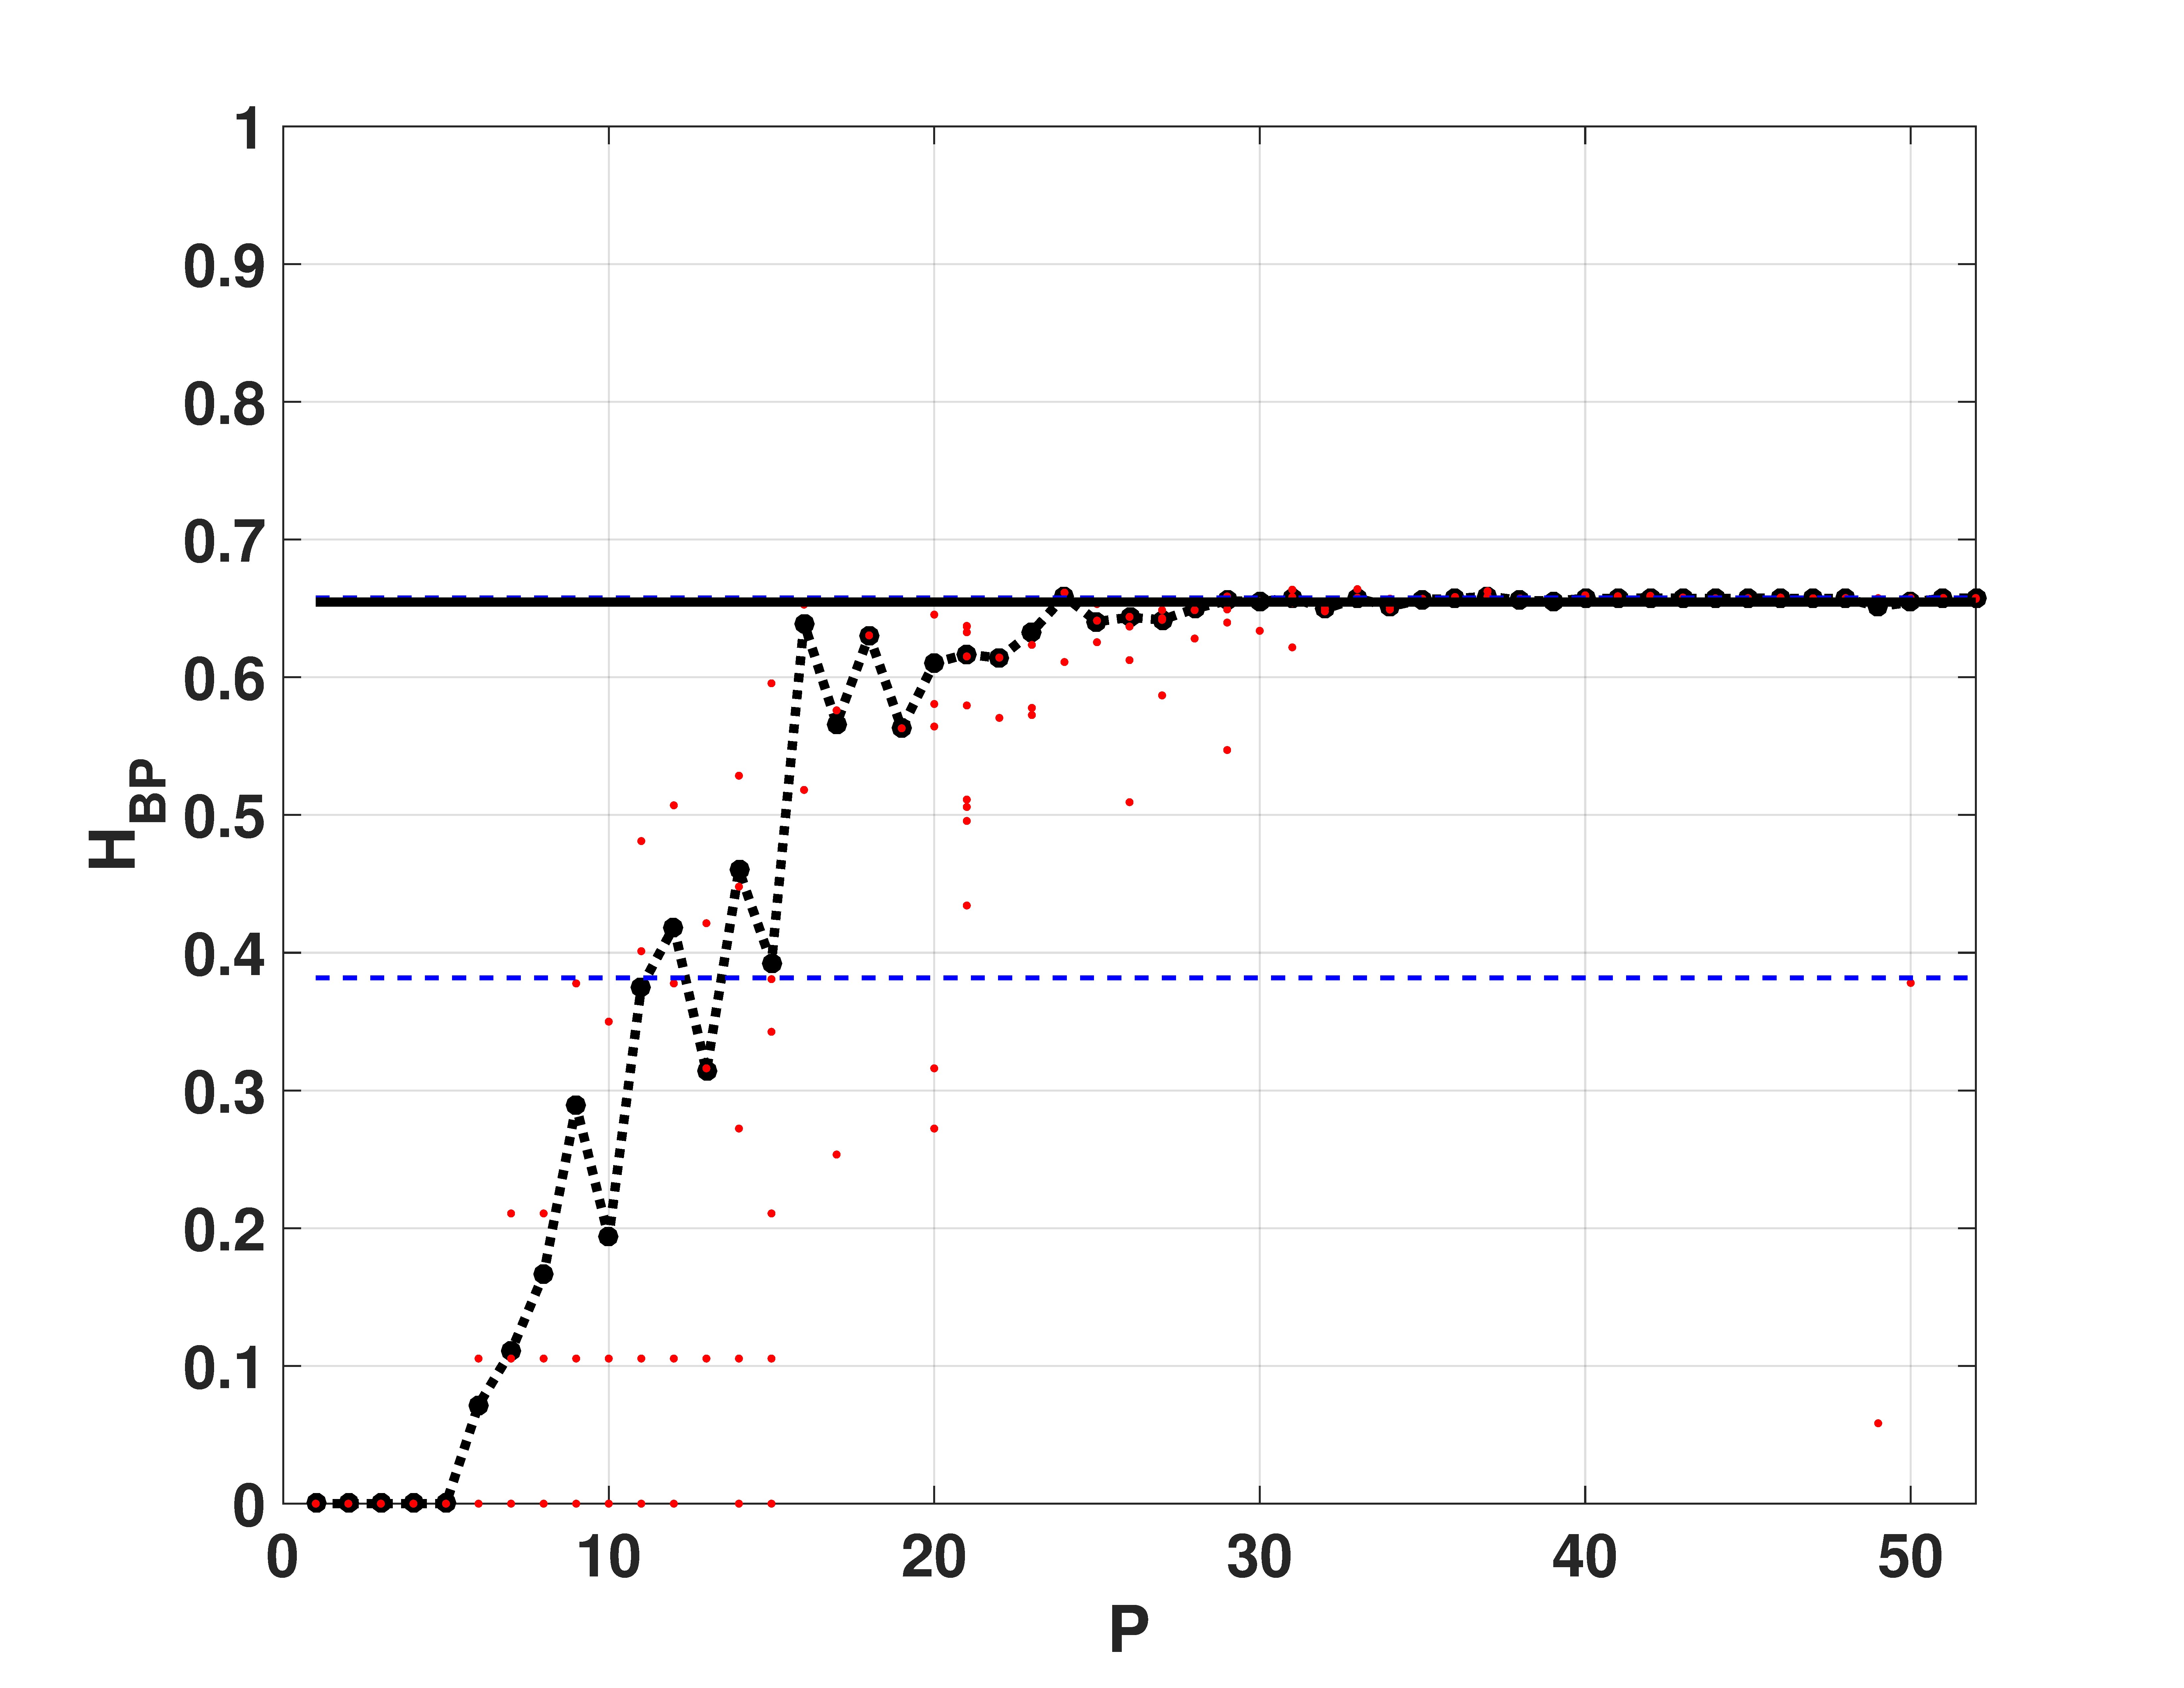
\includegraphics[width=.32\textwidth]{Hbp_Switch}
	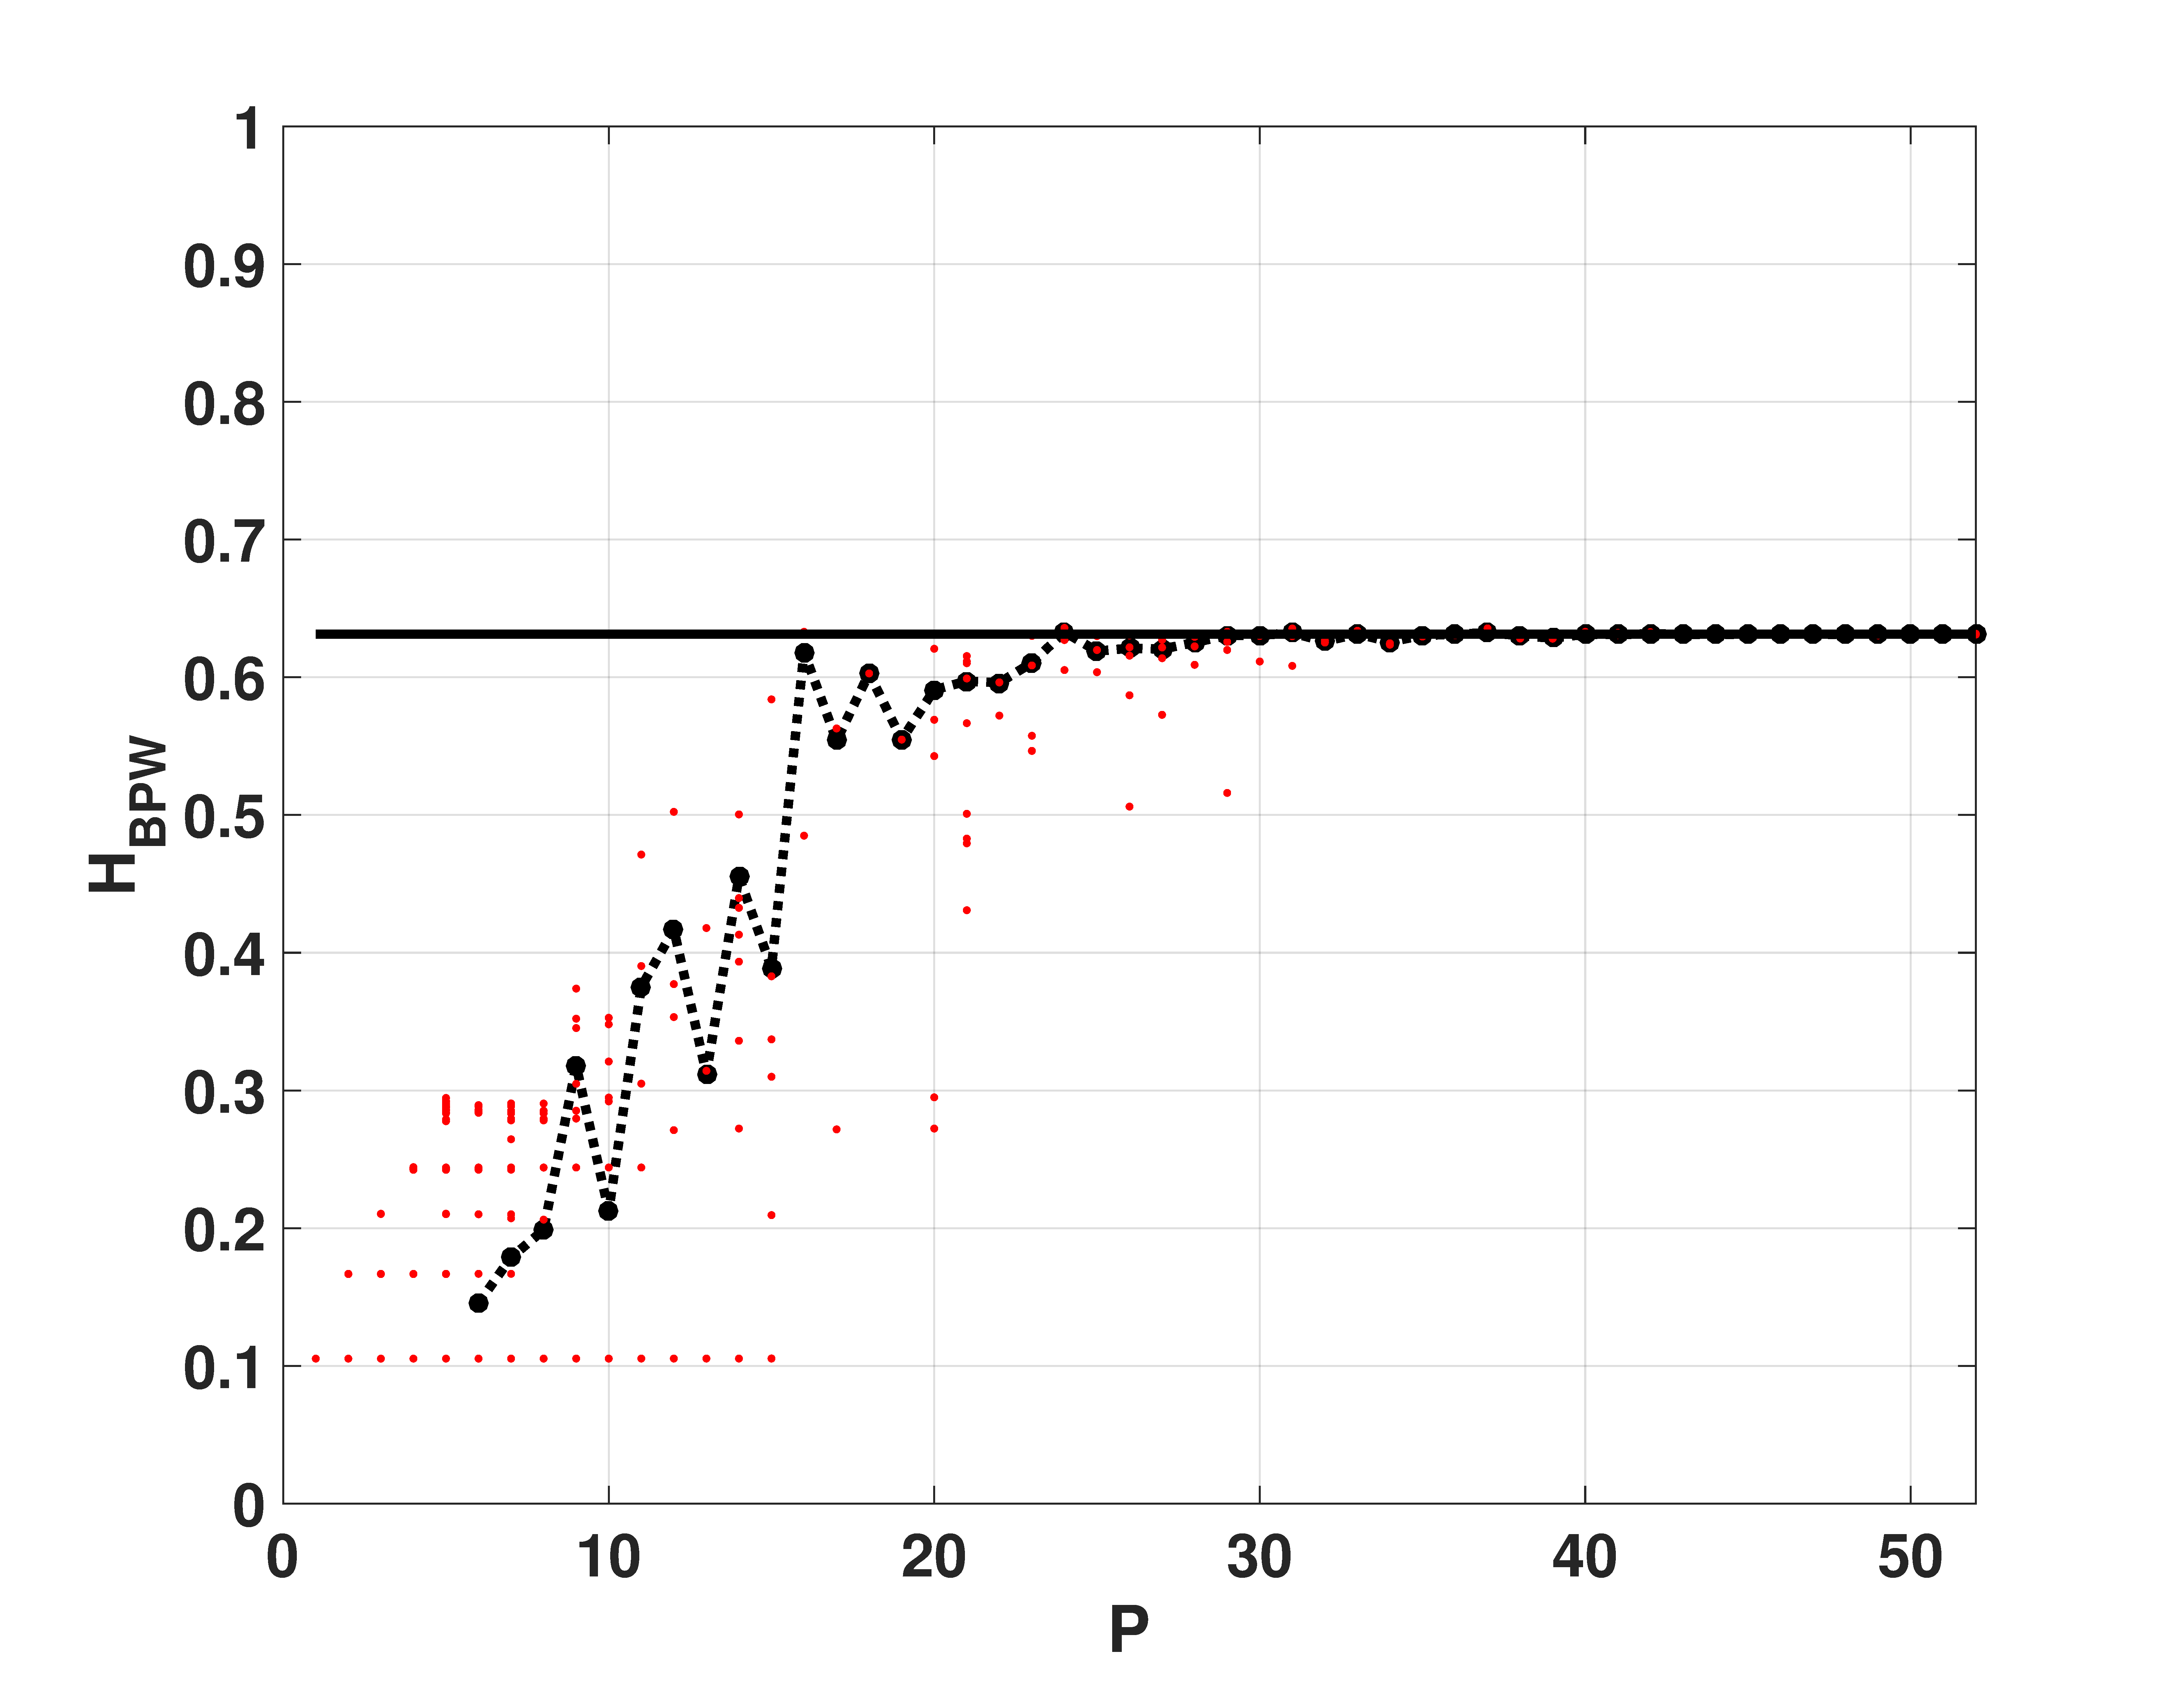
\includegraphics[width=.32\textwidth]{Hbpw_Switch}
	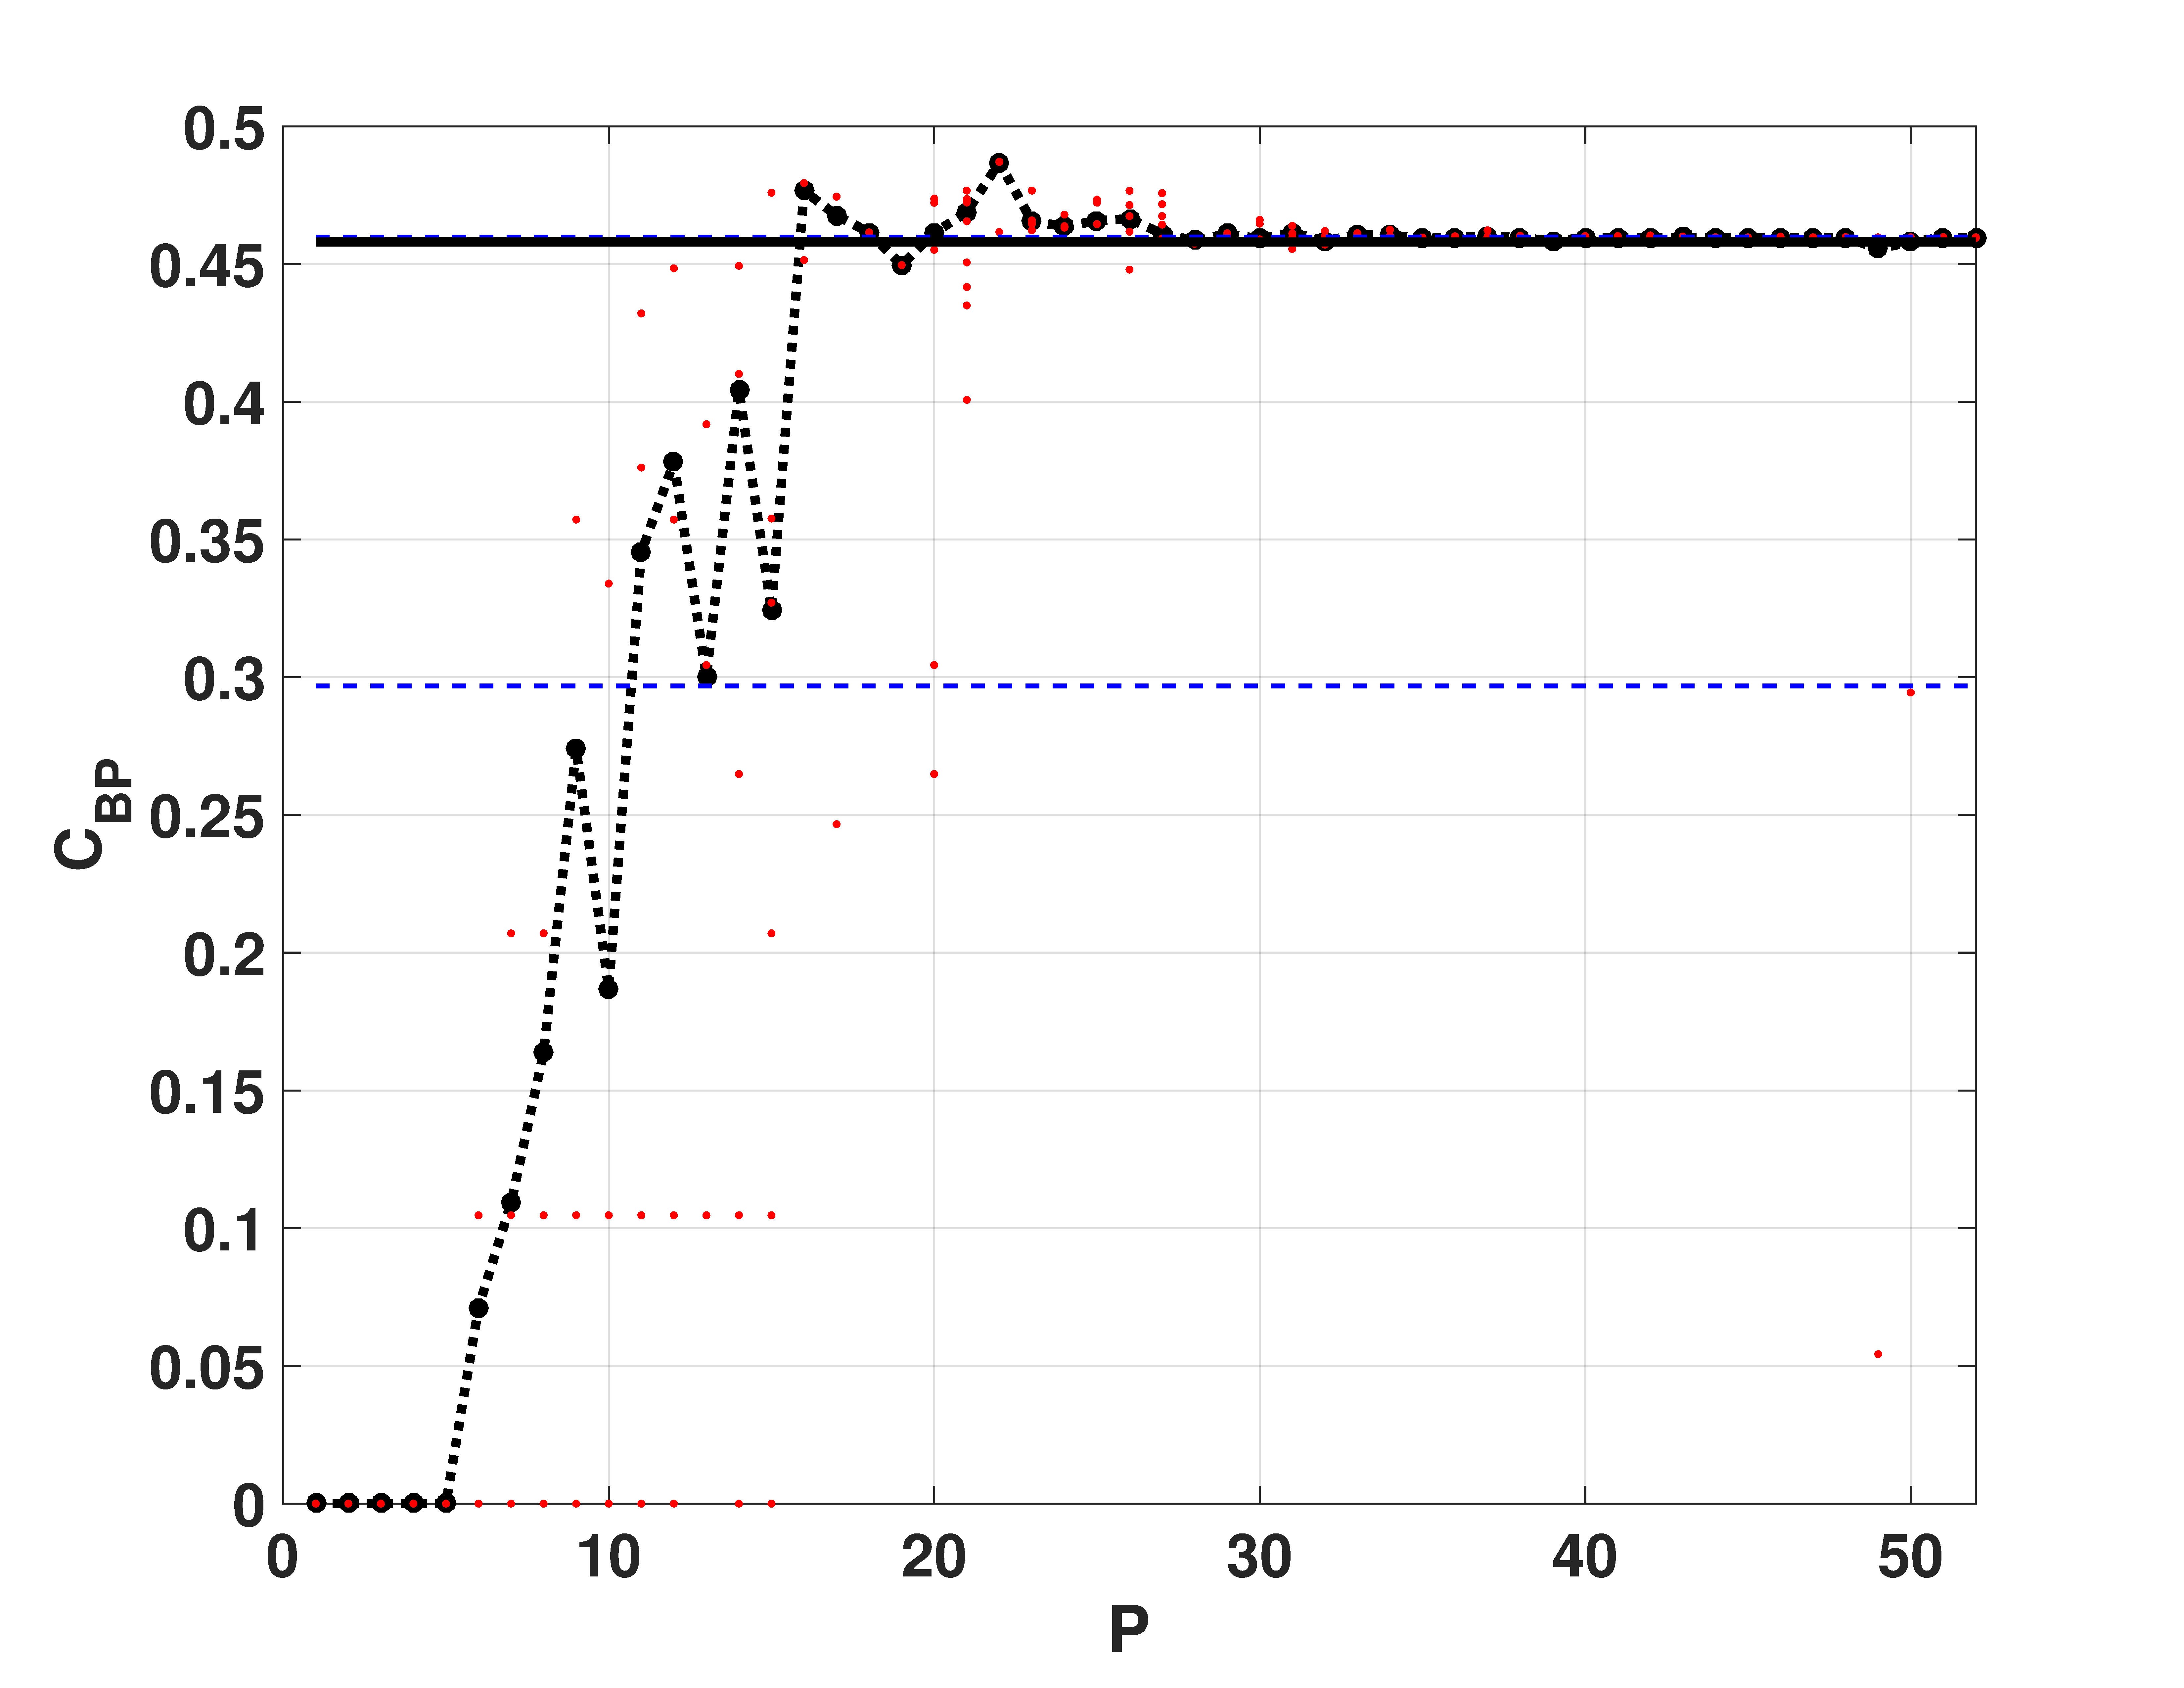
\includegraphics[width=.32\textwidth]{Cbp_Switch}
	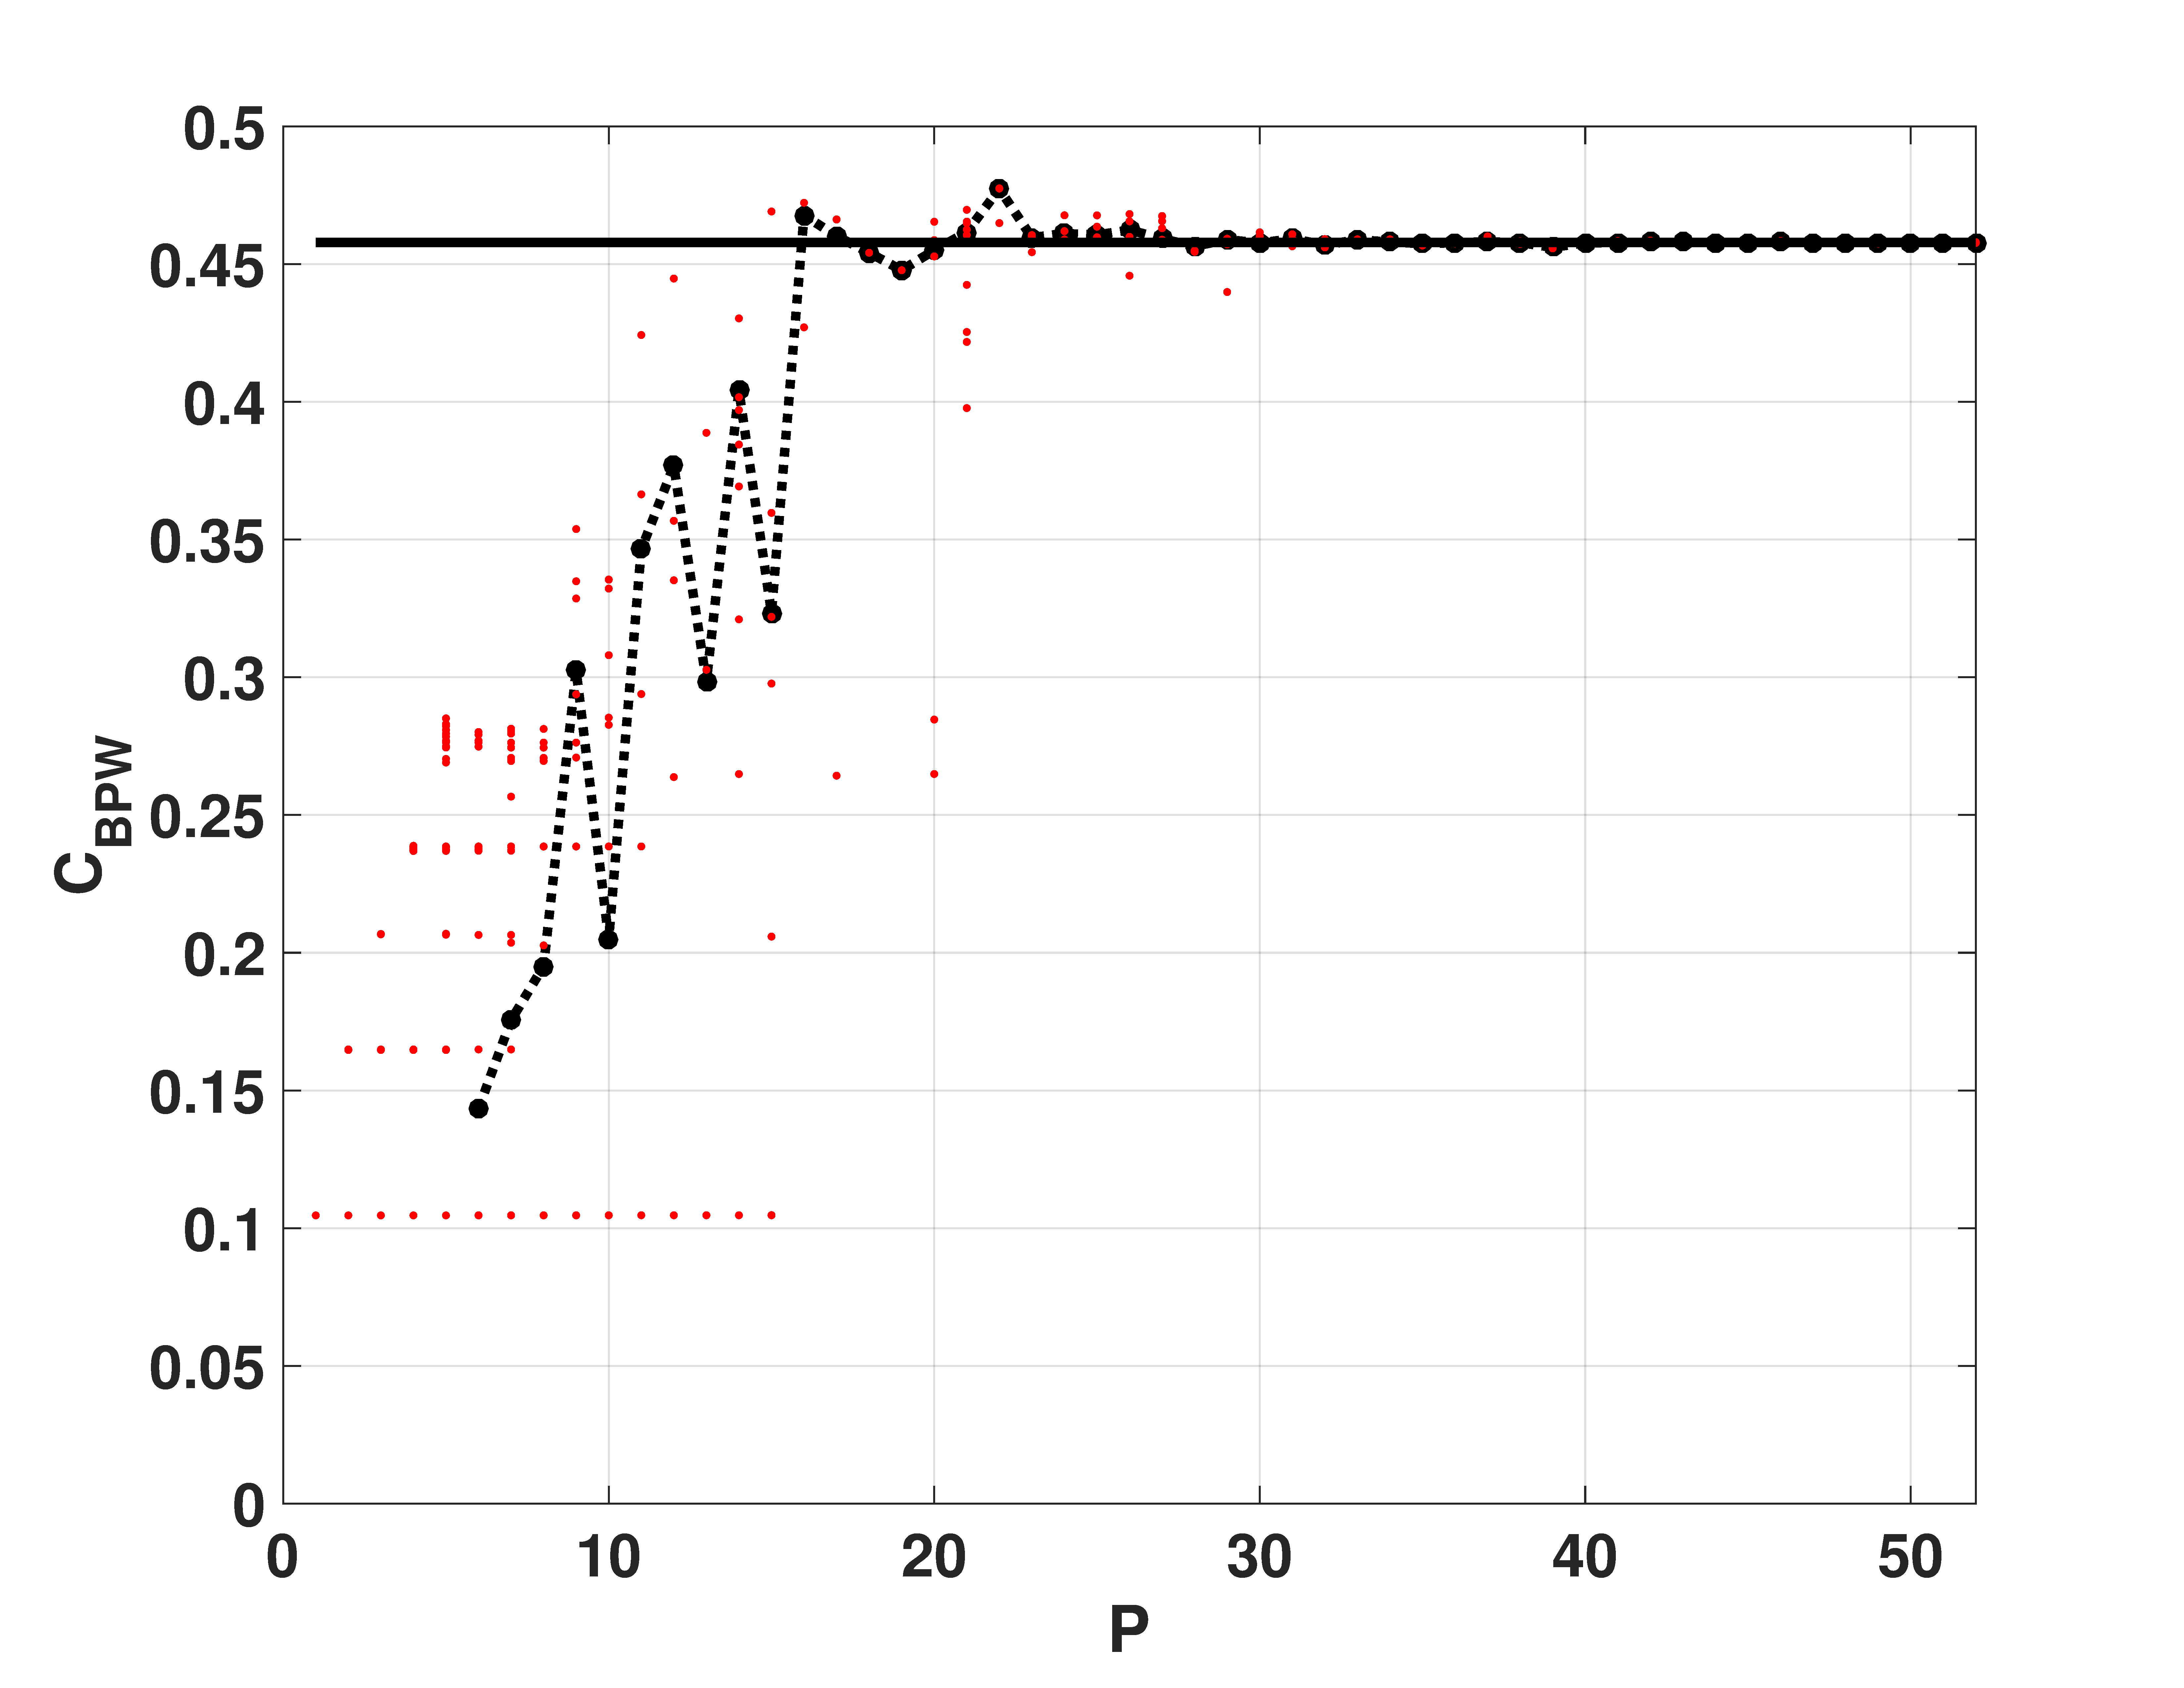
\includegraphics[width=.32\textwidth]{Cbpw_Switch}
	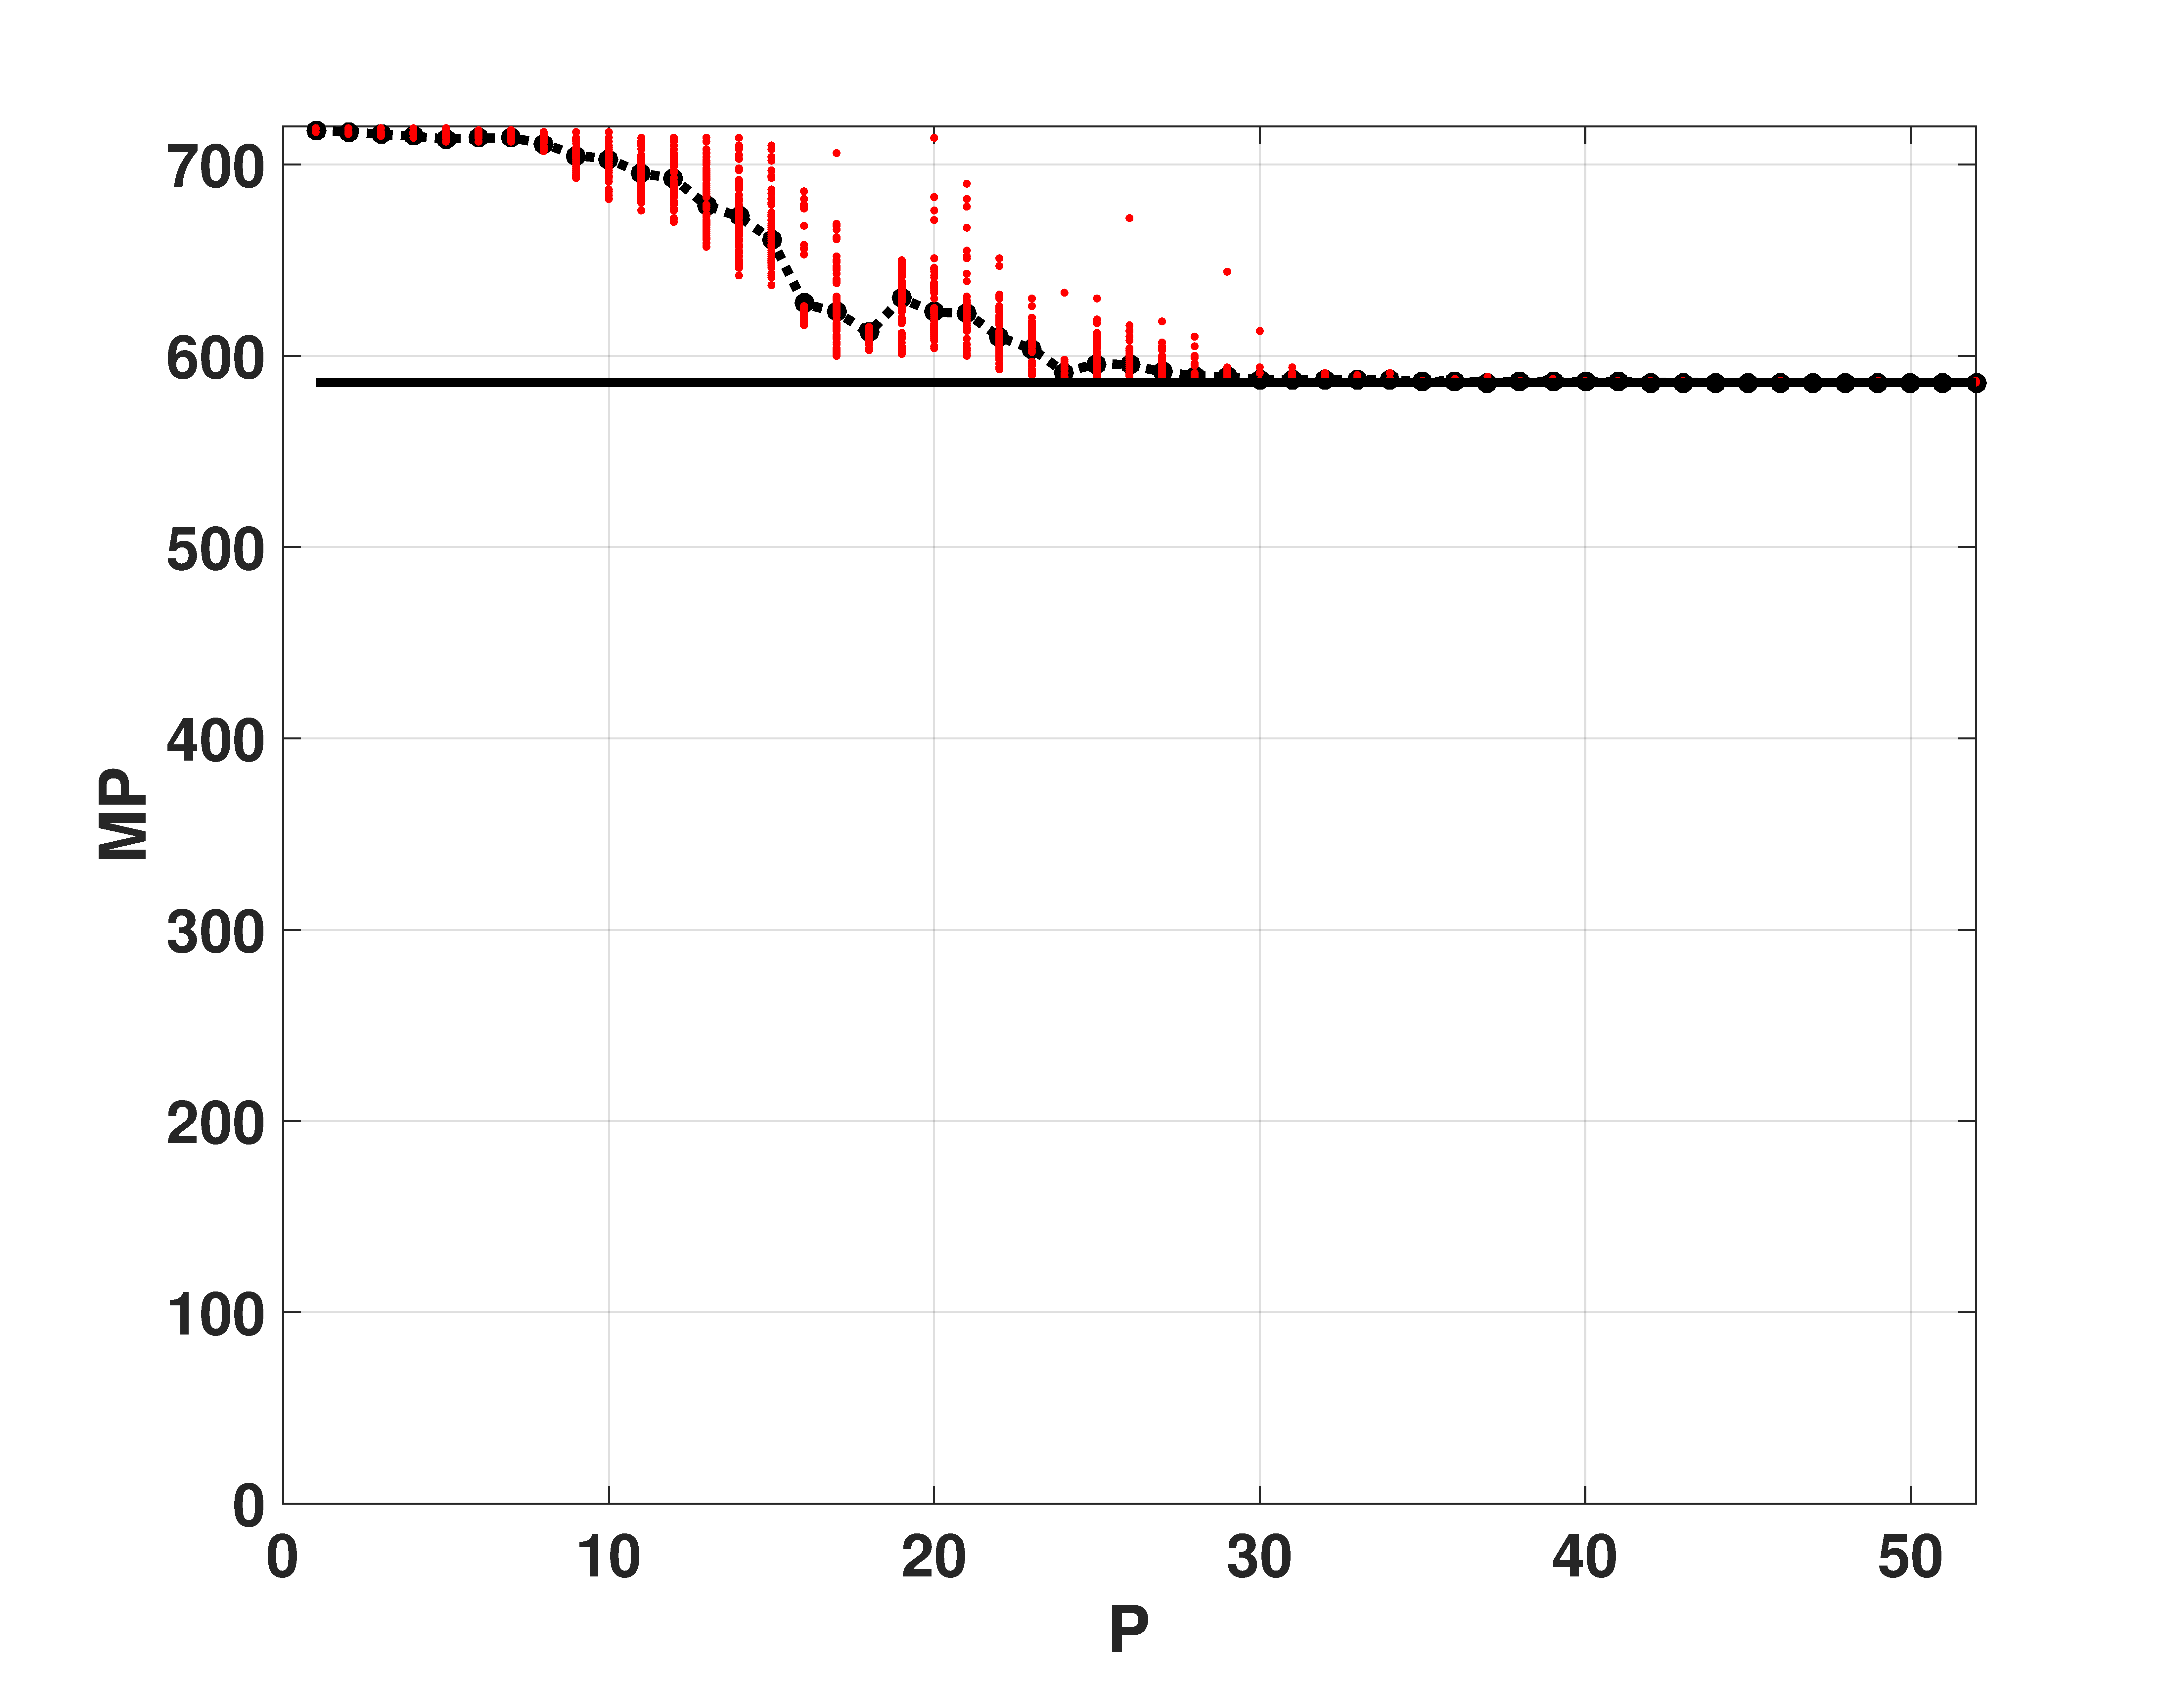
\includegraphics[width=.32\textwidth]{MP_Switch}
	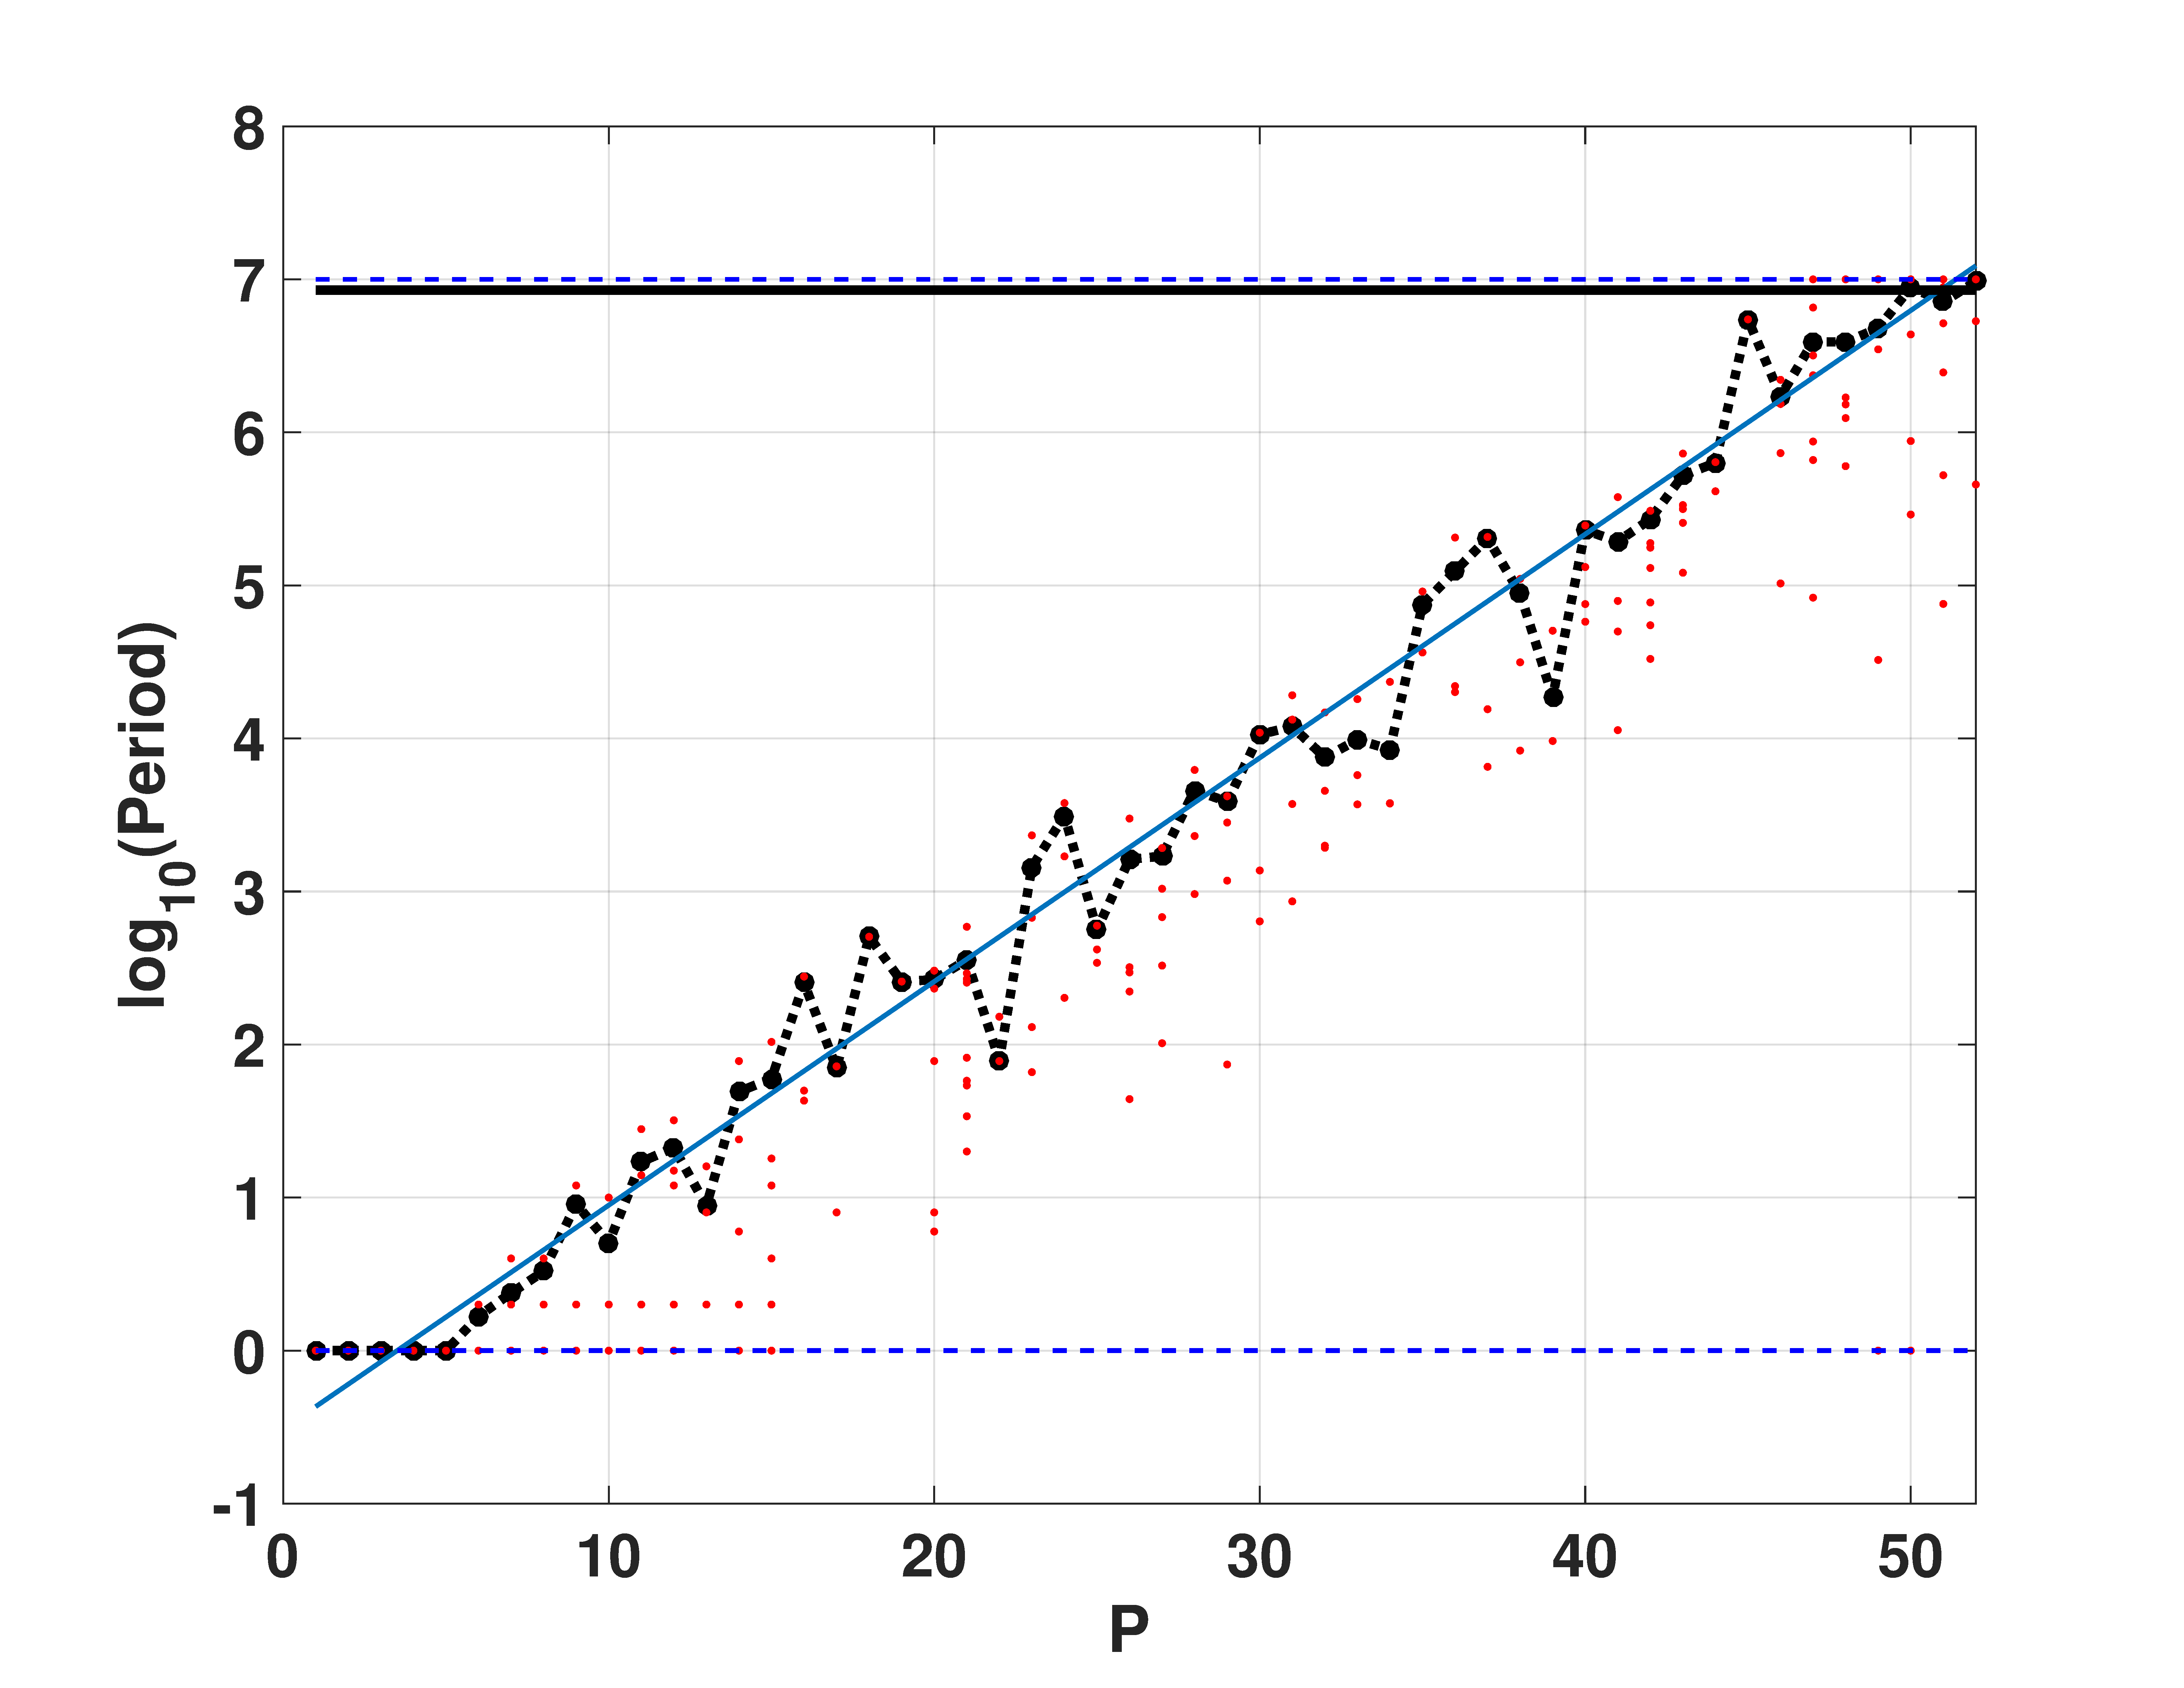
\includegraphics[width=.32\textwidth]{Period_Switch}
	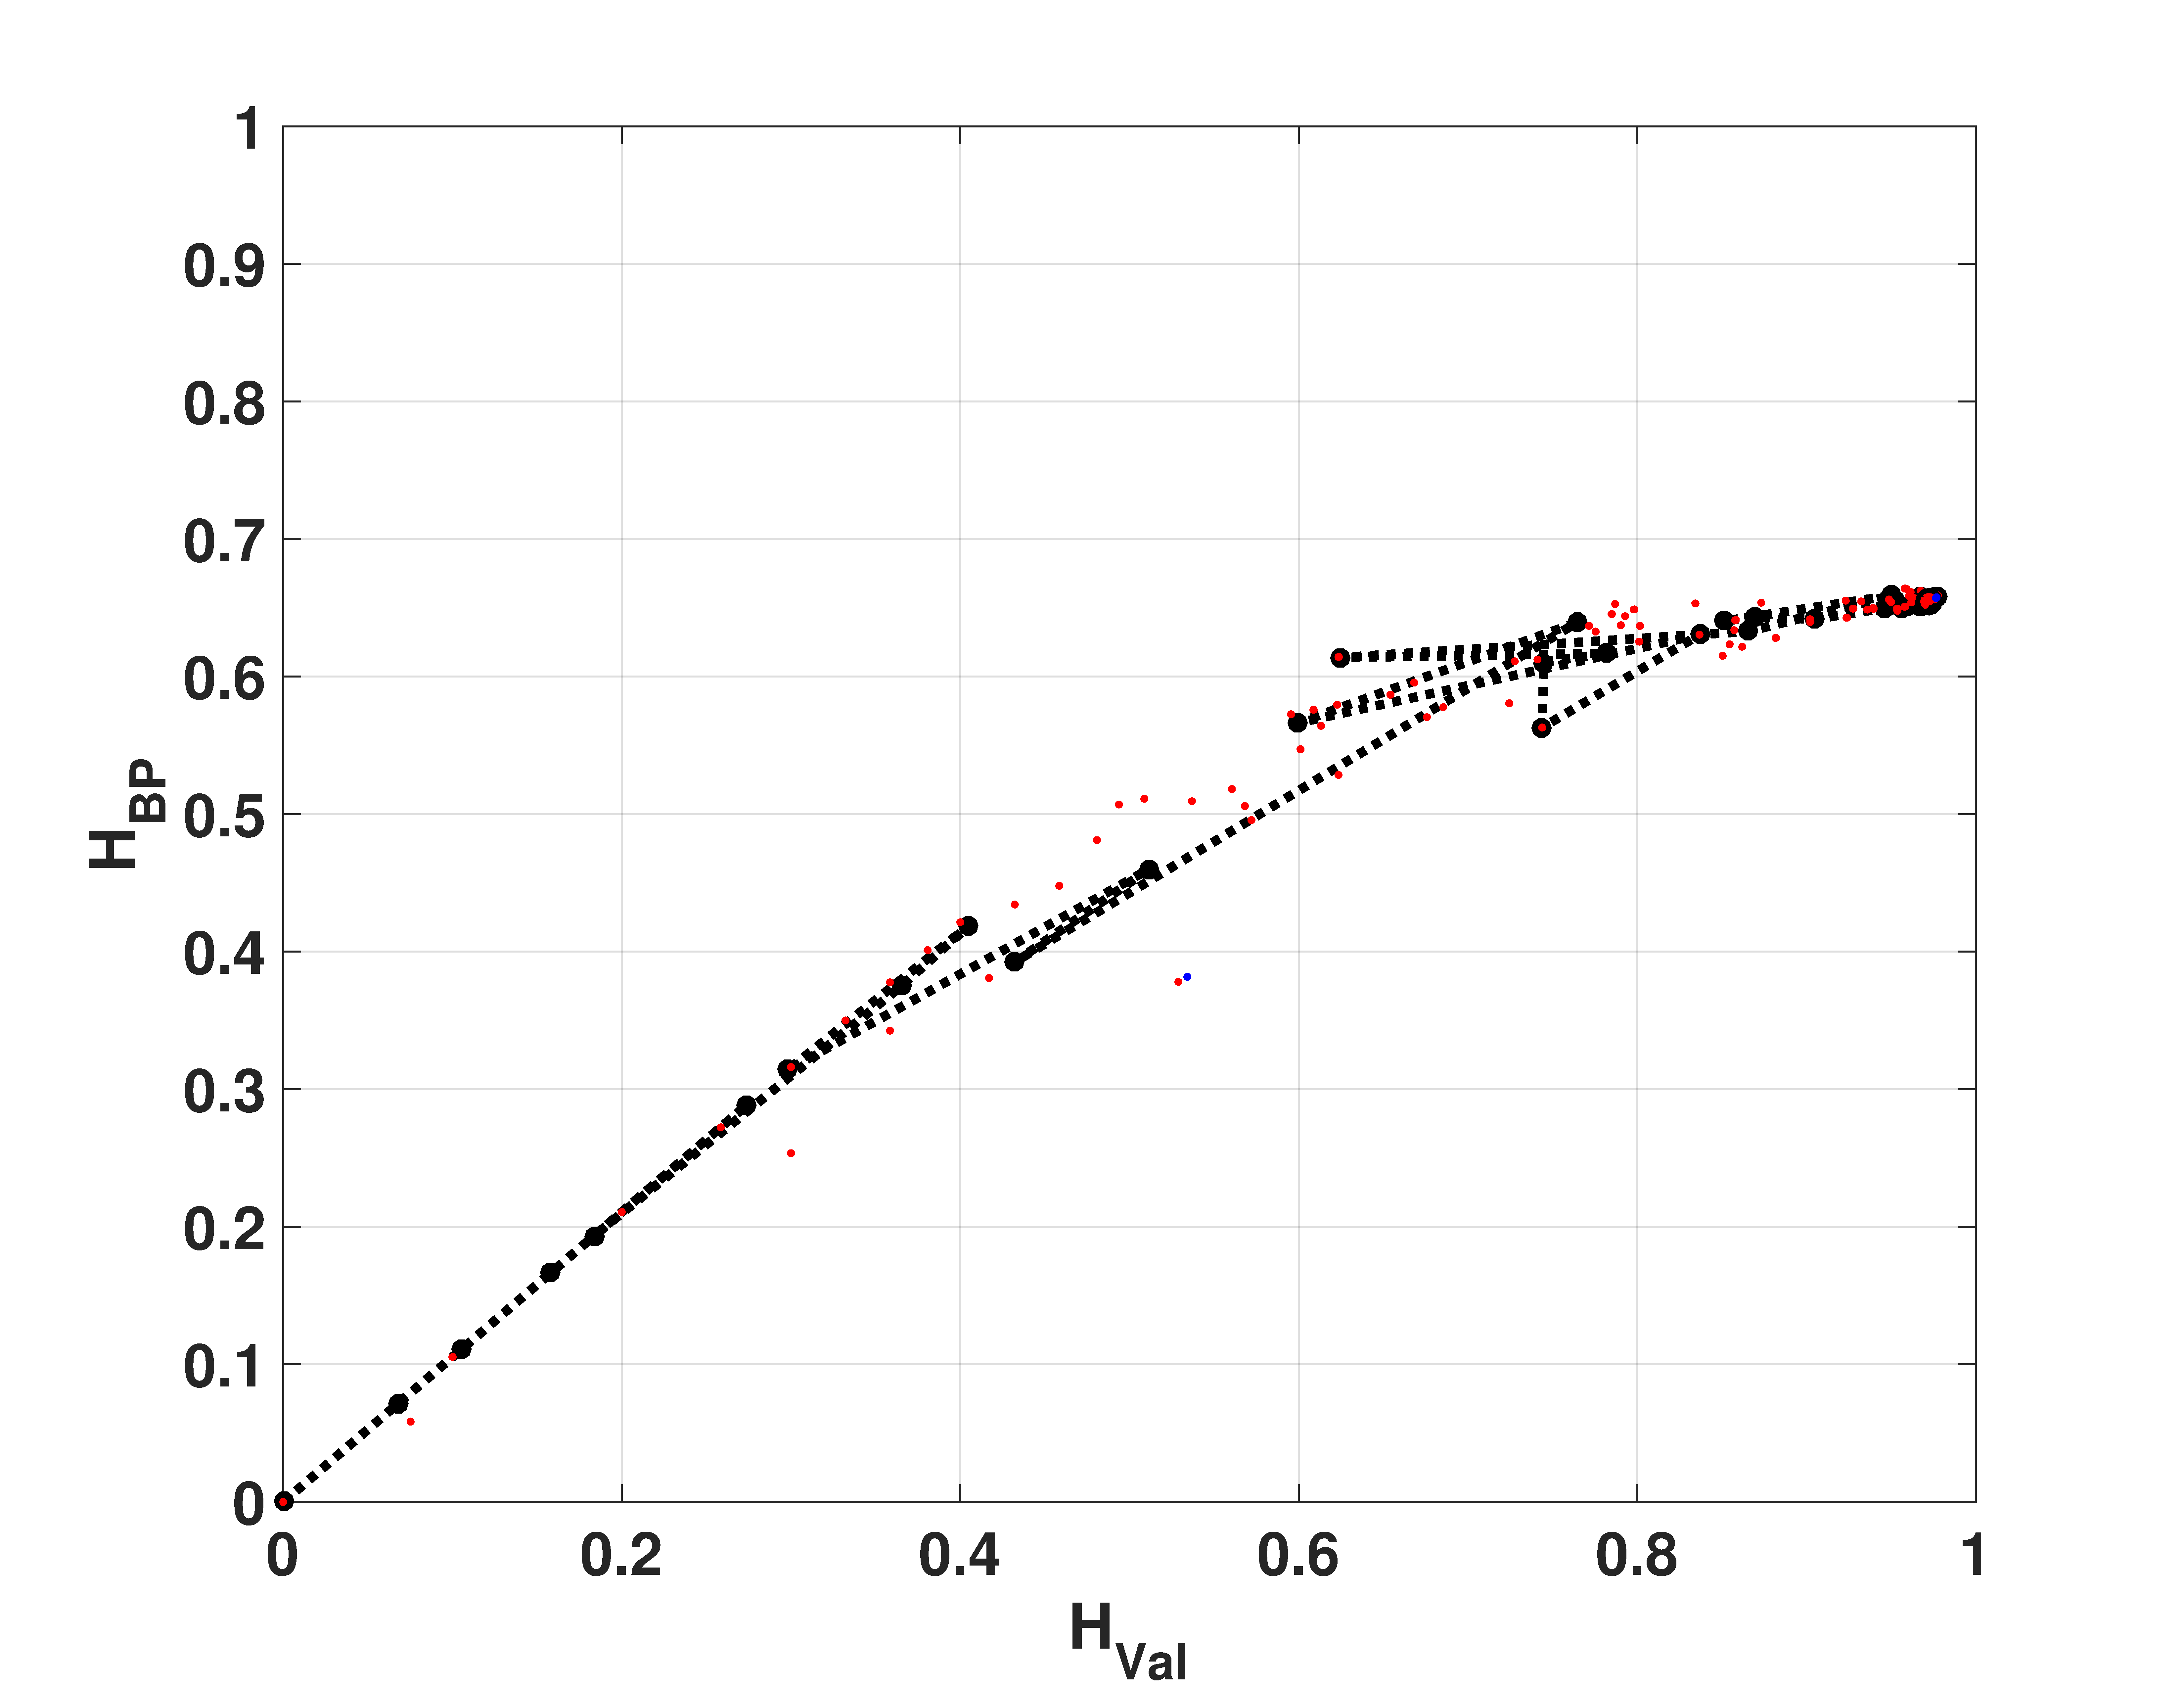
\includegraphics[width=.32\textwidth]{HbpHval_Switch}
	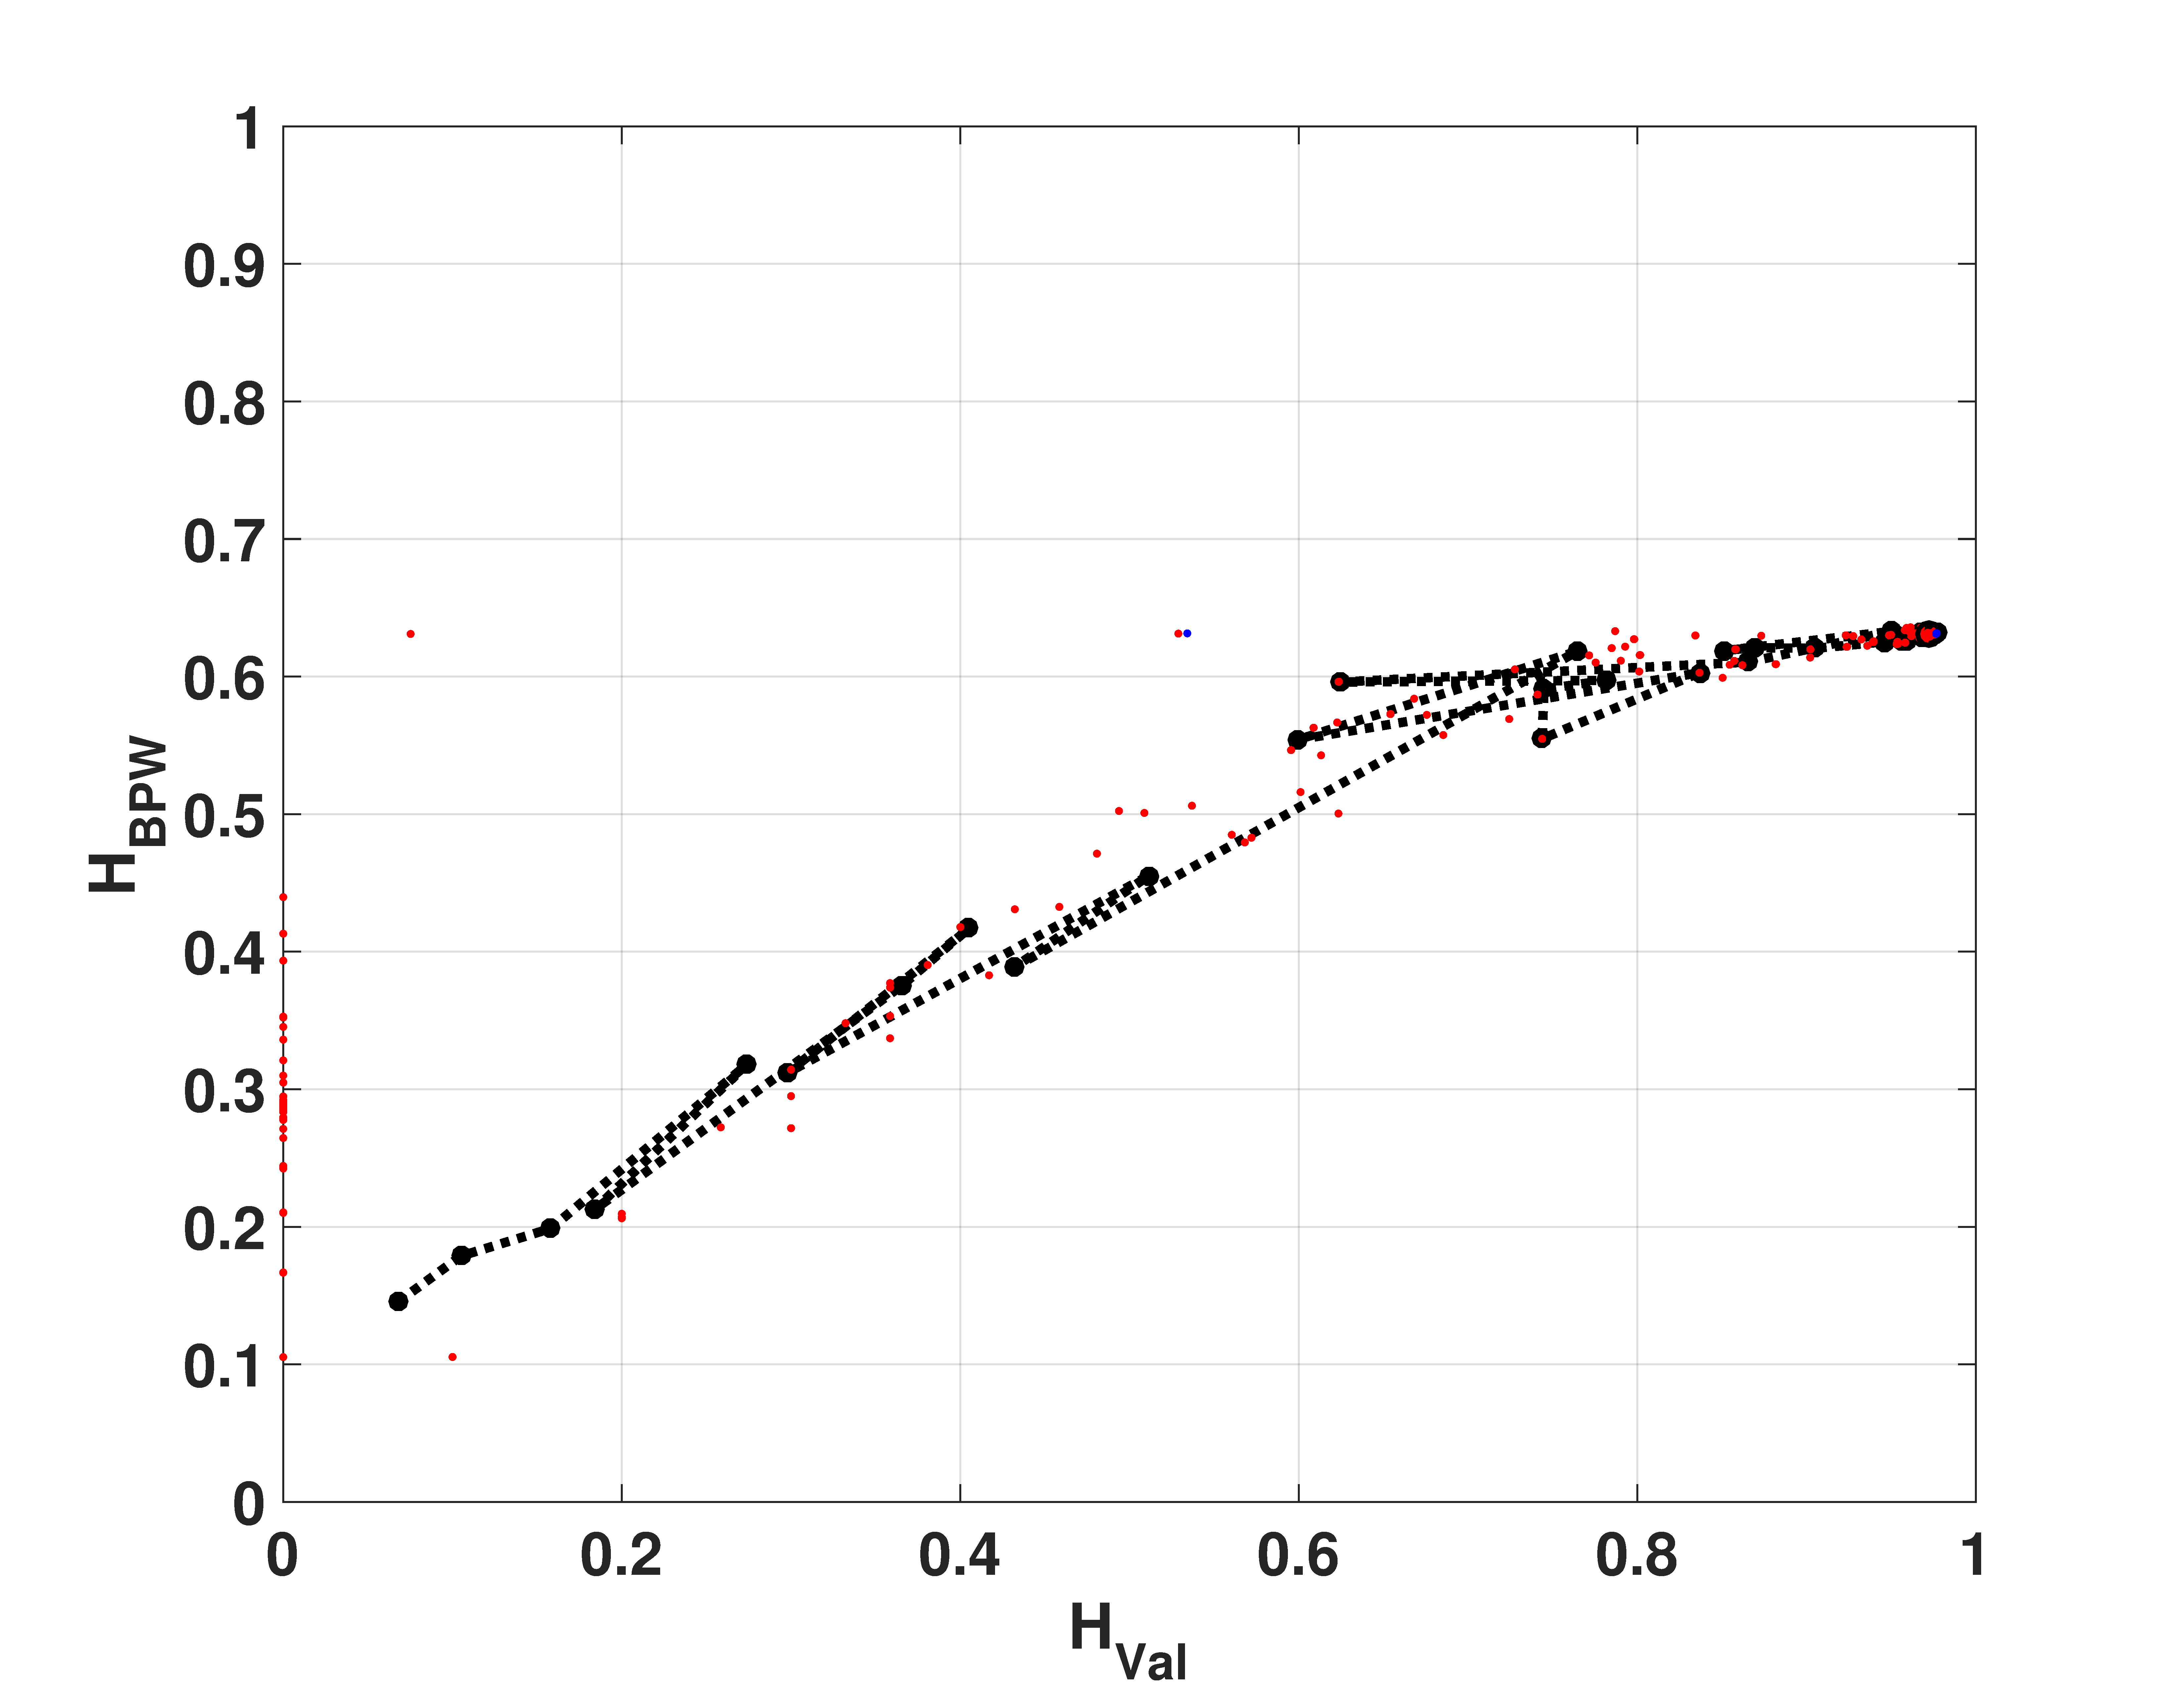
\includegraphics[width=.32\textwidth]{HbpwHval_Switch}
	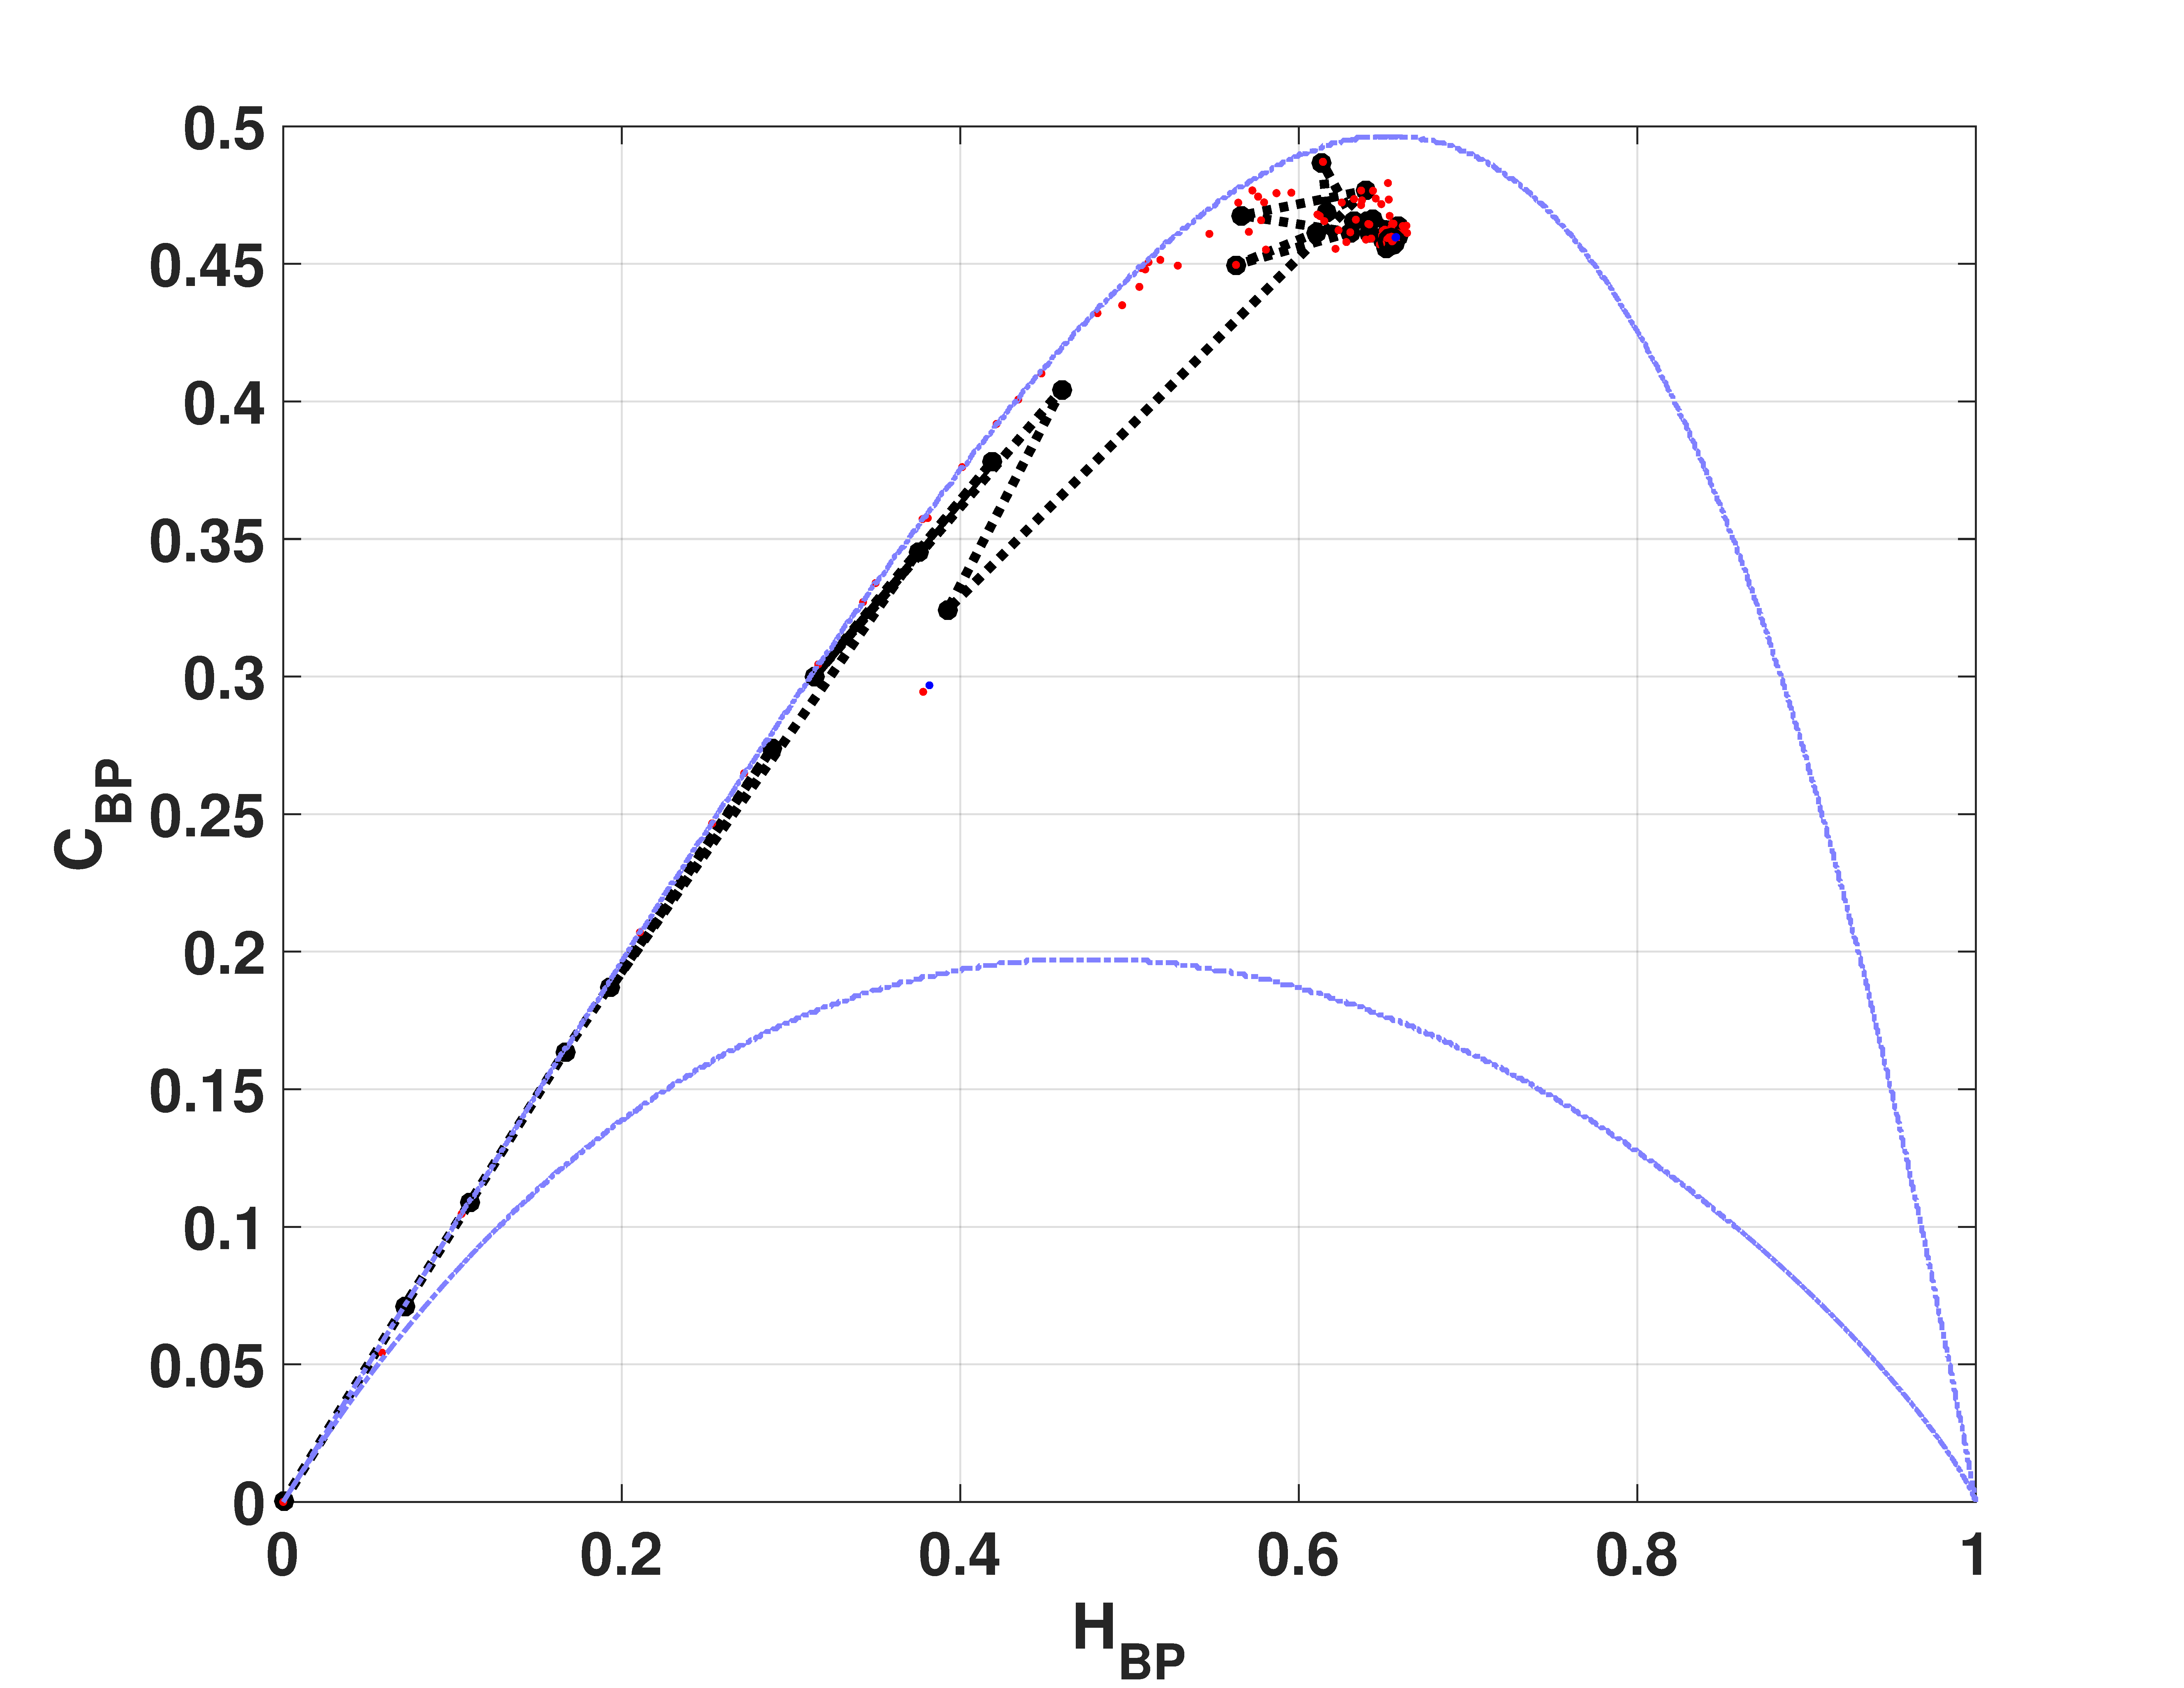
\includegraphics[width=.32\textwidth]{CbpHbp_Switch}
	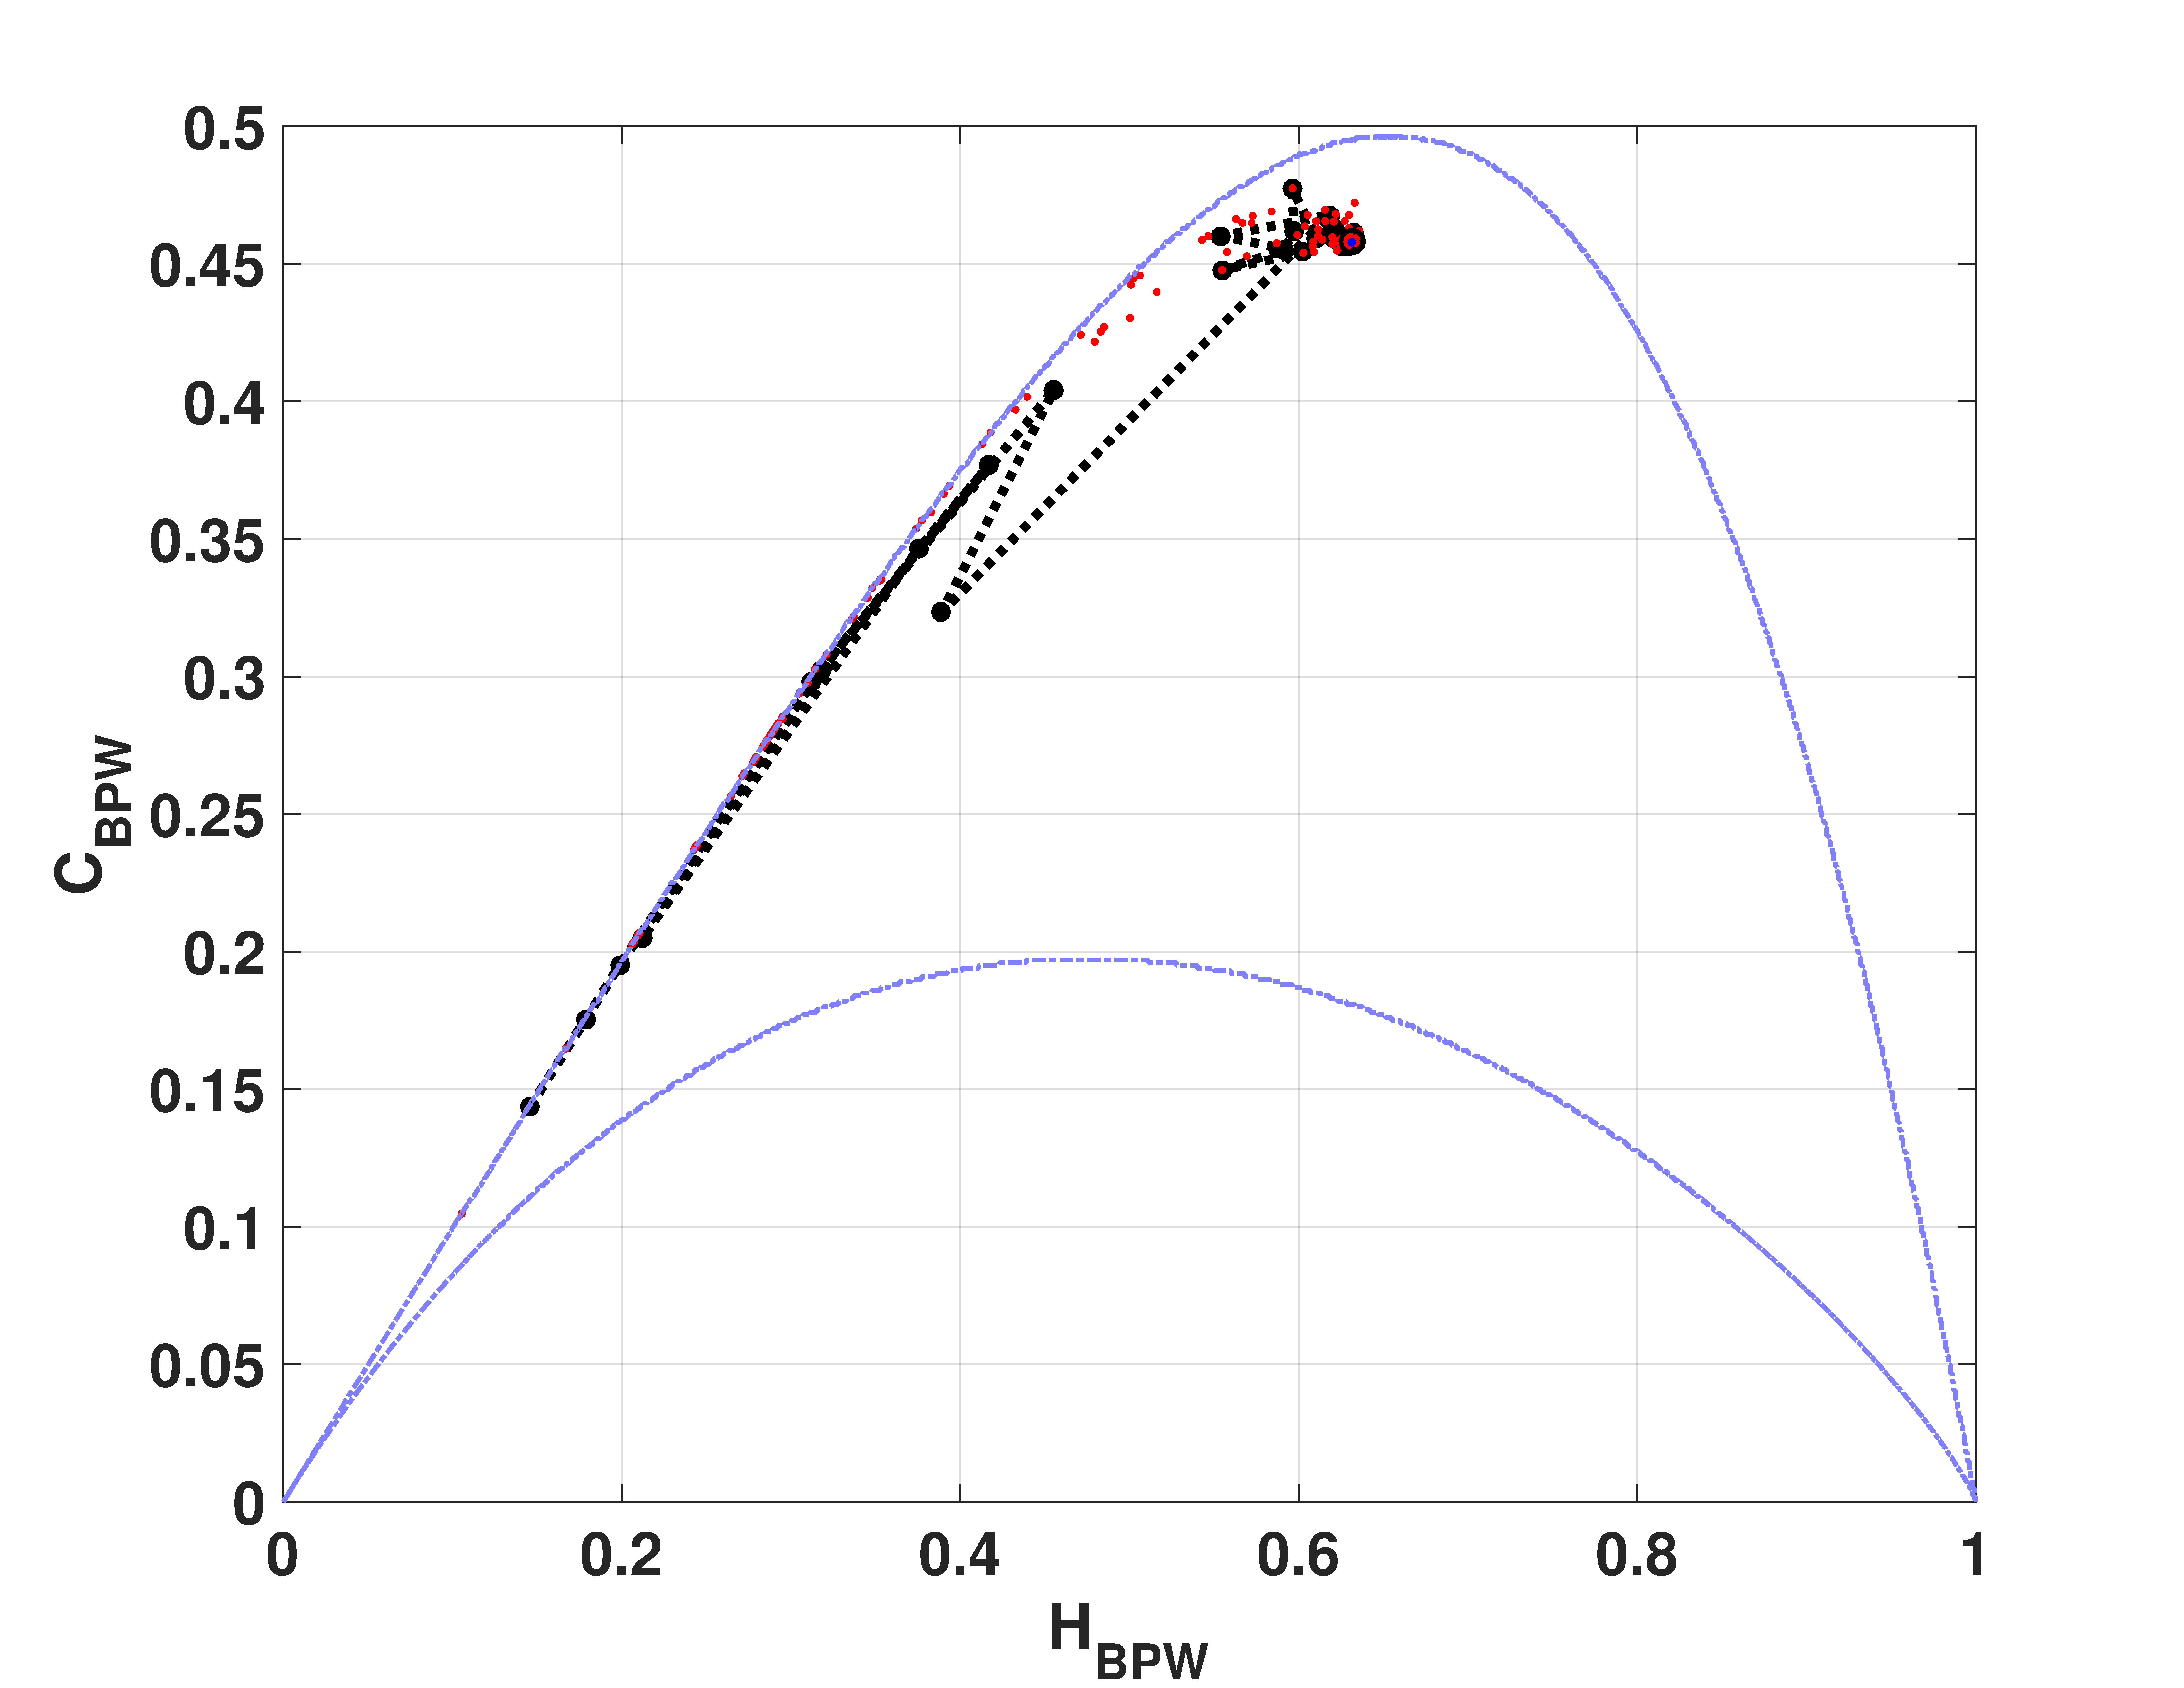
\includegraphics[width=.32\textwidth]{CbpwHbpw_Switch}
	\caption{Statistical properties of EVEN, obtained by skipping the values in the odd position of the time series of  SWITCH,  using binary representation: (a) $H_{hist}$ vs $P$ (b) $H_{BP}$ vs $P$ (c) $C_{BP}$ vs $P$ (d) Number of missing ordering patterns $MP$ vs $P$. In Figures (a) to (d) dashed line correspond to floating point numbers. (e) representation in the $H_{hist},H_{BP}$ plane in the the binary numerical system.  The star represents the state for floating points numbers. (f) representation in the $H_{BP},C_{BP}$ plane.  The star represents the state for floating points numbers.  } \label{fig:seqparbin}
\end{figure}